
\documentclass{report}           %% ceci est un commentaire (apres le caractere %)
%\usepackage[ landscape, margin=1in]{geometry}

\usepackage[utf8]{inputenc}
\usepackage[english]{babel}
\setlength{\parskip}{1em}
\renewcommand{\baselinestretch}{1.6}

\usepackage{geometry}
 \geometry{
 a4paper,
 total={170mm,245mm},
 left=20mm,
 top=30mm,
 }
 
\usepackage{relsize}
 
\usepackage{amsthm}
\usepackage{array}
\usepackage{amsmath}
\usepackage[ruled,vlined,linesnumbered,noresetcount]{algorithm2e}
\usepackage{algpseudocode}
\usepackage{dsfont}
\usepackage{tabu}
\usepackage{graphicx}
\graphicspath{ {img/} }
%\graphicspath{ {figures/} }
\usepackage{float}
\usepackage[justification=centering]{subfig}
\usepackage[colorlinks]{hyperref}
\usepackage{hyperref} 
\hypersetup{
    colorlinks=true,
    linkcolor=blue,
    filecolor=magenta,      
    urlcolor=cyan,
}
%\usepackage{algorithm}
%\usepackage{algpseudocode}
\usepackage{algorithm2e}
\usepackage{wrapfig}
\usepackage{listings}
\usepackage{caption}
%\usepackage{array,multirow,makecell}
%\setcellgapes{1pt}
%\makegapedcells

\usepackage{tabularx}

 %\renewcommand{\familydefault}{\sfdefault}
 
% \renewcommand{\familydefault}{\rmdefault}

\usepackage{lmodern}
\begin{document}



%\maketitle\thispagestyle{empty}

\begin{abstract}
Our work revolves around the recognition of both hands  gesture in Real time using the kinect sensor and machine learning . At first we acquired depth image of the kinect , using its advantage of depth  data we were able to detect And perform gesture by  Considering that the minimum depth from the sensor  is the hand region , since the hand gestures are  usually held in front of  the body  , this  allow us to track the hand and also it gives  the user more  mobility around the sensor rather than working in a certain closed and predefined range  , then we have developed an algorithm for gesture classification using SURF (Speeded up robust features )descriptor with features quantization using Bag of Visual words approach from depth image , a second algorithm was developed to meet  real time requirement for such  application  is Fourier descriptor , these two algorithms were used to classify various Gestures by two Machine Learning algorithms (Support vector Machine and  Nearest-Neighbor classifier )       
\end{abstract}


%content
\tableofcontents
%\listoffigures

\begin{quote}
 
\centering

    {
\huge 

GENERAL  INTRODUCTION 

}
\end{quote}


\vspace{1.5cm}

Hand gesture recognition  has gotten and still getting the researchers' attention and focus especially with the current HCI ( Human computer interaction ) evolution that provided Hardware -software  combination that is fast and suitable to interact with humans for a better HCI experience , and since there is a high need of silent communication using sign language for people with speech or  hearing  deficiencies/difficulties or in some cases both , additionally , there are situations when silent communication is preferred : for example , during a surgery,  a doctor may gesture to the nurse for assistance ,Hence making a real time  hand gesture recognition system has become inevitable.

Traditionally , gesture recognition requires high quality stereoscopic cameras with complicated computer vision algorithms to recognize hand signals ,which usually doesn't end to be as interactive as required and of course it requires extensive and expensive setup. but thanks to Microsoft  Kinect, we now can have  an inexpensive  sensors  that helps in having a good user experience in real time .

Microsoft released the first Beta of the Kinect software development kit for Windows 7. This SDK was meant to allow developers to write Kinecting apps by using Microsoft Visual studio including features like accessing Low-level streams from the depth sensor , RGB camera sensor   as well as skeletal  tracking, however,  there  is no hand  specific  data  available for  gesture   recognition,   although    it   includes   information  of the  joints   between  hands   and  arms.

Previous   researches  \ref{chapter1}  on  computer   vision  and hand   detection   have established   solid  groundwork    for gesture   recognition, but  only  a  few  Kinect based   systems  were  developed   for  HGR    and  only  a  few  gestures were recognized . and that is  the main motive behind This Project basing our work on a novel method for contact-less HGR using both bare hands or just  one hand, the system is able to detect hand gestures  made by user , track it  in a range of [ 80 cm until 3meters ] long  and  recognize the meanings of gestures, the real power of the system is its ability to give high accuracy  despite the lighting  conditions,   skin color, clothing,  and background.

Two major approaches were implemented in this project ,  based on Features extractions and Machine learning , the first approach  is  Surf(Speeded up robust features) Features Trained with both K-means And SVM(Support Vector Machine ) , the second approach  based on Fouriere  shape descriptor  features using Nearest neighbor Classifier . Note more details about the implementation are going to be discussed in Chapter \ref{hgr} .

For these purposes we will be studying  Some of the famous Image local Descriptors like ( Sift and Surf )  in chapter  \ref{descriptors}   to familiarize with some of their key words like ( \textbf{keypoints localization , orientation assignment , keypoint descriptor} ..)  and  then  reviewing shape feature extraction using Fouriere descriptor and Covariance matrix approach in  section [\ref{FDT}] , and Finally we are going to Explore  Some of the main ideas behind the success of our learning algorithms and their robustness for our HGR system  in chapter [\ref{ML}].

In the next Chapter we will go through Some of the famous approaches in  Literature about HGR  System , hoping this Chapter will give  credits  to researchers behind a lot of success for this Project .







\chapter{LITERATURE SURVEY}

\section{introduction:}

According to the World Federation of Deaf (WFD) \ref{} there are 70 million deaf people in world, whereas the world population in 2012 exceeded 7 billion \ref{}[4] , this number has got the power to make research in the field of machine vision  over  the  past  decade rich  approaches .
A  more  recent   technology  for gesture   recognition  is to  incorporate   the  information   of object   distances,   or depths,   normally   captured   by a 3D camera,   or a set  of cameras  that  produce 3D images and that it is Technology that will be used in this project  .It is also a contact-less  user interface,   in contrast   to glove based   devices  or handhold   remote  sensor .
With the kinect DEpth Sensor stream data it is now possible to make recognize and  translate sign language in to speech and / or text in order to facilitate better communication between normal hearing and hearing impaired people. This is usually called Sign Language Recognition (SLR) which  aim  to automatically understand meaning of a sequence of signs from sign language without involvement of human interpreter \ref{ }. This chapter covers key aspects of SLR Literature.

\section{ Sign  Language Recognition}  

the SLR system can be divided into 4 important  steps , Data acquisition and feature extraction and finally Feature combination and Sign recognition .however in whats the next  we will cover Two important approaches that both  belongs to the first step ( Data acquisition ) :\\

Device based :
in  1991 Tomoichi Takahashi  \ref{ } developed a system for real time SLR  using Device based approach such system required the user to wear gloves that were connected to computer for transmission of hand signal ,experiments showed that 34 of 46 gestures of the Japanese Kana manual alphabet were recognized correctly \ref{}.
 A wireless glove that was designed by Ryan Petters  \ref{}in 2002, sensed hand movements involved in sign language and then transmitted them wirelessly to portable device, that displayed translated signs as lines of text \ref{} [31].
 

vision based :
 This approach  \ref [32] here  feature extraction was done using color camera for recognition of ASL. Two experiments were run: the first required from the signer to wear colored gloves, while the second used hand’s skin color for feature extraction \ref [32]. The extracted features were used as input for HMM algorithm that was used during sign recognition phase. The first experiment attained 99\% word accuracy while the second 92\% \ref [32] .
 
 Two experiments were carried out also in \ref [33] on a SLR system that combined computer vision and HMM for recognition of sentence level continuous ASL. Both systems were tested with forty (40) words from ASL, where in first systems single camera was mounted on desk to track user’s hands and achieved 92\% word accuracy, while in second system the user had to wear a cap worm in which camera was mounted and the achieved accuracy was 97\%  \ref [33].




The presentation of all works related to SLR is not the intention of this section and more can be found on  \ref{}[27],\ref{} [36] and \ref{ }[39]. 

The following section present works that employed Kinect device for building SLR systems.Where we are going to discover The main ideas behind our project 

\section{Gesture Recognition Using Kinect :}

in \ref{} Zhou Ren et al presents a gesture recognition System using Kinect Sensor accompanied with a novel distance metric called Finger-Earth Mover’s Distance (FEMD) to measure the hand shape dissimilarities, which not only achieves better performance than Shape Context, in terms of accuracy (a 93.9\% mean accuracy) and efficiency (0.5004s). 
A more recent approach followed by Daniel in \ref{} uses Kinect skeletal tracking for features extraction. Other features were derived from skeletal tracking and finally 8-features were used for unique description of each sign. Sign recognition employs nearest neighbor algorithm that tries to find closest matching of performed sign within a group of stored sings  For a dictionary of 14 homemade signs the system achieves an accuracy of 95\% \ref{} [47]. 

in \ref{} This paper presents an effective way of exploring depth information for hand gesture recognition. using  SIFT keypoint descriptor to extract local keypoint features
over depth images which is attempted for the first time in gesture recognition research. The recognition technique is inherently robust against scaling, rotation, and illumination conditions.  the features were  quantified  and clustered , and finally fed to  An SVM to be trained .\\


\textbf{ Insipired HGR of This Project : }


\textbf{With \ref{} And \ref{} } we inspired our most work dedicated for this Project , we take advantage of  depth and Skeletal Tracking  data generated by Kinect to detect the hand and track it  in a range of [ 80 cm until 3 meters ] long  .
After detection of hand, we uses SURF Descriptor for Features detection and Extraction then we  cluster these vectors via a bag-of-features (BOW) model , these features are then Fed to an SVM with two different Kernels Linear and RBF kernel .

on the other hand unlike most system that like \ref{} that uses HMM ,  we proposed and tested a method for static hand gesture recognition.using  Fourier shape  descriptor which proved to be a very efficient way for feature extraction. It provided a set of invariant features for each image and by using a small number of features , we Found NN classifier to give faster and better results for Fourier descriptor .


\section{syntax}

....
\\
....
\\
....


\newpage
\section{Conclusion}

We can Summarize The process Used in SLR literature as the following:

Getting data from a sign performing  it can either be Device based or / and Vision approach , then features
involved in sign making must be extracted and finally combination of features must be analyzed 

\begin{figure}[H]
\centering
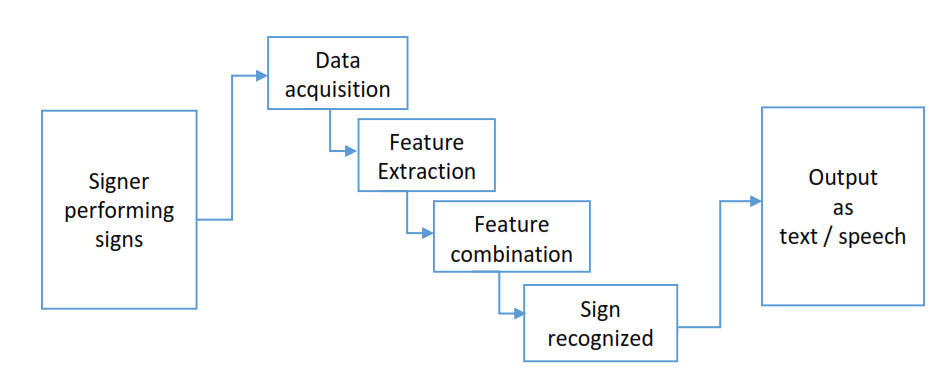
\includegraphics[width=0.8\textwidth]{img/SLR.PNG}
\caption{  Process of SLR }
\label{fig:SLR}
\end{figure}

In the next Chapter we will cover Image Descriptors As the Second Step of Our HGR System ,we will go through some of the important Feature of these Descriptor and how it can benefits our purposes in making Robust and Accurate HGR System . 

\chapter{Descriptors}

\section{introduction}

Over the last decades, image feature detectors and descriptors have become popular tools in the computer vision community and they are being applied widely in a large number of applications. Image representation , image classification and retrieval  , object recognition and matching  3D scene reconstruction , motion tracking   texture classification , robot localization, all rely on the presence of stable and representative features in the image. Thus, detecting and extracting the image features are vital steps for these applications.
Hence The need for a Descriptor that can detect and extract Features 
and Since our HGR system needs a Features detector that can be stable in most cases which will  full fill our need to Recognize the Gesture performed by the user .\\

\textit{Note : The Definition of SIFT  Descriptor might be long and has a lot of Definitions because Sift is considered as the most  powerful and widely used local descriptor in object recognition and image classification Hence the Literature focus on it  , and as a guarantee  to ensure the understanding of  Sift definition and key words  we will summarize all Sift's  Definition  IN THE END OF EVERY SECTION }

\section{Definitions and Principles:}

\subsection{Global and Local Features}
the following definition was given by M. Hassaballah et al in \ref{}. 
In the global feature representation, the image is represented by one multidimensional
feature vector, describing the information in the whole image.\\
In other words, the global representation method produces a single vector with values that
measure various aspects of the image such as color, texture or shape. Practically, a
single vector from each image is extracted and then two images can be compared by
comparing their feature vectors.\\ For example, when one wants to distinguish images
of a sea (blue) and a forest (green), a global descriptor of color would produce quite
different vectors for each category. In this context, global features can be interpreted
as a particular property of image involving all pixels.
This property can be color
histograms, texture, edges or even a specific descriptor extracted from some filters
applied to the image \cite{h}.\\ On the other hand, the main goal of local feature representation
is to distinctively represent the image based on some salient regions while
remaining invariant to viewpoint and illumination changes. Thus, the image is represented
based on its local structures by a set of local feature descriptors extracted
from a set of image regions called interest regions (i.e., keypoints) as illustrated in
Fig.\ref{fig:Ft1} Most local features represent texture within the image patch.

\begin{figure}[H]
\centering
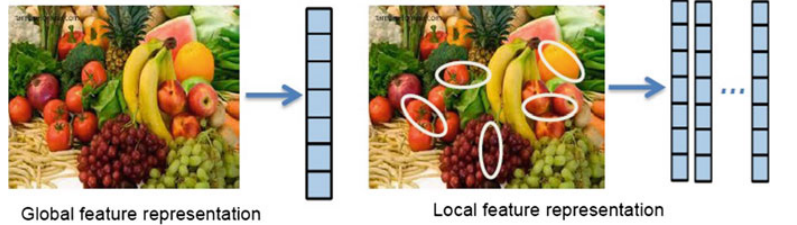
\includegraphics[width=0.9\textwidth]{img/features.PNG}
\caption{ Global and local image features representation }
\label{fig:Ft1}
\end{figure}

Generally, using what kind of features might greatly depend on the applications
on hand. Developers prefer the most discriminative ones. For example, a person with
a bigger nose and smaller eyes, and a person with a smaller nose and bigger eyes
may have similar mug shot in terms of histogram or intensity distribution. Then, local
features or the global pattern distilled from local feature clusters seem to be more
discriminative. Whereas, for very large datasets in the web scale image indexing
application, it is appropriate to consider global features. Also, global features are
useful in applications where a rough segmentation of the object of interest is available.
The advantages of global features are that they are much faster and compact
while easy to compute and generally require small amounts of memory.\\ Nevertheless,
the global representation suffers from well known limitations, in particular they
are not invariant to significant transformations and sensitive to clutter and occlusion.\\In some applications, such as copy detection, most of the illegal copies are very  similar to the original; they have only suffered from compression, scaling or limited
cropping. In contrast, the advantage of local features is their superior performance \cite{i}. Meanwhile, using local features for large scale image search have much higher performance than global features provide \cite{k}.\\ Besides, as the local structures are more distinctive and stable than other structures in smooth regions, it is expected to be more useful for image matching and object recognition.\\ However, they usually require a significant amount of memory because the image may have hundreds of local features.\\ As a solution for this problem, researchers suggest aggregating local image descriptors into a very compact vector representation and optimizing the
dimensionality reduction of these vectors \cite{k}


\subsection{Characteristics of Feature Detectors}

Tuytelaars and Mikolajczyk \cite{MM} define a local feature as \textit{ “it is an image pattern
which differs from its immediate neighborhood”.} Thus, they consider the purpose of
local invariant features is to provide a representation that allows to efficiently match
local structures between images. That is, we want to obtain a sparse set of local
measurements that capture the essence of the underlying input images and encode
their interesting structures. To meet this goal, the feature detectors and extractors
must have certain properties keeping in mind that the importance of these properties
depends on the actual application settings and compromises need to be made. The
following properties are important for utilizing a feature detector in computer vision
applications:
\begin{itemize}
\item Robustness, the feature detection algorithm should be able to detect the same feature
locations independent of scaling, rotation, shifting, photometric deformations,
compression artifacts, and noise
\item Repeatability, the feature detection algorithm should be able to detect the same
features of the same scene or object repeatedly under variety of viewing conditions.
\item Accuracy, the feature detection algorithm should accurately localize the image
features (same pixel locations), especially for image matching tasks, where precise
correspondences are needed to estimate the epipolar geometry.
\item Generality, the feature detection algorithm should be able to detect features that
can be used in different applications.
\item Efficiency, the feature detection algorithm should be able to detect features in new
images quickly to support real time applications.
\item Quantity, the feature detection algorithm should be able to detect all or most of the
features in the image. Where, the density of detected features should reflect the
information content of the image for providing a compact image representation.
\end{itemize}

\textbf{in this project We are going to use Local Features( descriptors) For its Efficiency and scale , Rotation  Invariant }\\
\section{Spectra descriptors :}
\subsection{SIFT - Scale Invariant Feature Transforms} \label{siftSection}

The Scale Invariant Feature Transform (SIFT) developed by Lowe \ref{} is the most well known method for finding interest points and feature descriptors, providing invariance to scale, rotation, illumination, affine distortion, perspective and similarity
transforms, and noise. Lowe demonstrates that by using several SIFT descriptors together to describe an object, there is additional invariance to occlusion and clutter. We provide some detail here on SIFT since it is well designed and well known.


\begin{enumerate}
\item Scale-Space Extrema Detection :
The first stage of computation must search over all
scales and image locations, but it can be implemented efficiently by using a difference of-Gaussian
function to identify potential interest points that are invariant to scale and
orientation.
\item Keypoint localization :
At each candidate location, a detailed model is fit to determine
location, scale, and contrast. Keypoints are selected based on measures of their
stability.
\item Orientation assignment :
One or more orientations are assigned to each keypoint
location based on local image properties. All future operations are performed relative
to the assigned orientation, scale, and location for each feature, providing invariance
to these transformations.
\item Keypoint descriptor  :
The local image gradients are measured at the selected scale
in the region around each keypoint, and transformed into a representation that allows
for local shape distortion and change in illumination.
\end{enumerate}

An important aspect of this approach is that it generates large numbers of features that
densely cover the image over the full range of scales and locations.\\ A typical image of size
500$\times$500 pixels will give rise to about 2000 stable features (although this number depends
on both image content and choices for various parameters).\\ The quantity of features is
particularly important for object recognition, where the ability to detect small objects in
cluttered backgrounds requires that at least 3 to 6 features be correctly matched from each
object for reliable identification.
For image matching and recognition, features are first extracted from a set of reference
images and stored in a database.\\ A new image is matched by individually comparing
each feature from the new image to this previous database and finding candidate matching
features based on Euclidean distance of their feature vectors.\\
The keypoint descriptors are highly distinctive, which allows a single feature to find its
correct match with good probability in a large database of features. 



\subsection{Scale-Space Extrema Detection :}
As described in [\ref{siftSection}], we will detect keypoints using a sequential filtering approach
that uses efficient algorithms to identify candidate locations that are then examined
in further detail.\\ The first stage of keypoint detection is to identify locations and scales that
can be repeatably assigned under differing views of the same object. Detecting locations
that are invariant to scale change of the image requires that we search for stable features
across all possible changes of scale, using a continuous function of scale known as scale
space (Witkin, 1983).\\
It has been shown by Koenderink (1984) and Lindeberg (1994) that under a variety of reasonable assumptions the only possible scale space kernel is the Gaussian function.
Therefore, the scale space of an image is defined as a function, L(x, y, $\sigma$), that is produced
from the convolution of a variable scale Gaussian, G(x, y,$\sigma$), with an input image, I(x, y):\\

L(x, y, $\sigma$) = G(x, y,$\sigma$) * I(x, y),


where * is the convolution operation in x and y, and

\begin{align*} 
 G(x, y,\sigma )  =\frac{1}{2\pi\sigma^2} e^\frac{-( x^2 -  y^2)}{2\sigma^2}  
\end{align*}

To efficiently detect stable keypoint locations in scale space, we have proposed (Lowe,
1999) using scale space peaks in the difference-of-Gaussian function convolved with the
image, D(x, y, $\sigma$), which can be computed from the difference of two nearby scales separated
by a constant factor k:
\begin{align}
D(x, y, \sigma) &= (G(x, y, k\sigma) - G(x, y,\sigma) * I(x, y)\\
                 &= L(x, y, k\sigma) - L(x, y, \sigma) .
   \end{align}               
                  
There are a number of reasons for choosing this function. First, it is a particularly
efficient function to compute, as the smoothed images, L  need to be computed in any
case for scale space feature description, and D can therefore be computed by simple image
subtraction.

\begin{figure}[H]
\centering
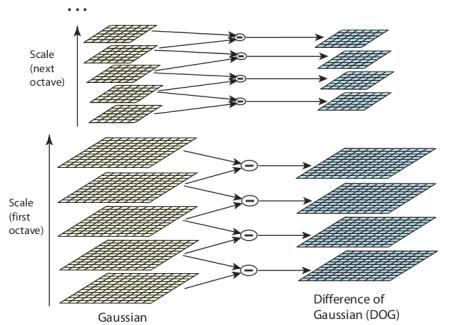
\includegraphics[width=0.8\textwidth]{img/sift_dog.jpg}
\caption{ DOG Principale .}
\label{fig:sift1}
\end{figure}

In addition, the difference-of-Gaussian function provides a close approximation to the
scale normalized Laplacian of Gaussian, $\sigma^2\nabla^2 G $
, as studied by Lindeberg (1994).\\Lindeberg
showed that the normalization of the Laplacian with the factor $\sigma^2$
is required for true scale invariance. In detailed experimental comparisons, Mikolajczyk (2002) found that the maxima and minima of $\sigma^2\nabla^2 G $  produce the most stable image features compared to a range
of other possible image functions, such as the gradient, Hessian, or Harris corner function.\\
The relationship between D and $\sigma^2\nabla^2G $
G can be understood from the heat diffusion
equation (parameterized in terms of $\sigma$ rather than the more usual t = $\sigma^2$):\\

\begin{align}
    \frac {\partial G} {\partial \sigma} = \sigma \nabla^2 G 
\end{align}




From this, we see that$\nabla^2$ G can be computed from the finite difference approximation to  $\frac{\partial G}{\partial \sigma }$ , using the difference of nearby scales at k$\sigma$ and $\sigma$ :\\


\begin{align}
      \sigma \nabla^2 G =   \frac {\partial G} {\partial \sigma} \approx   \frac {G(x,y,k \sigma) -  G(x,y,\sigma)}{ k \sigma - \sigma}  
\end{align}


and therefore,


\begin{align}
      G(x,y,k \sigma) -  G(x,y,\sigma)  \approx (k - 1)  \sigma^2\nabla^2G 
\end{align}

\begin{figure}[H]
\centering
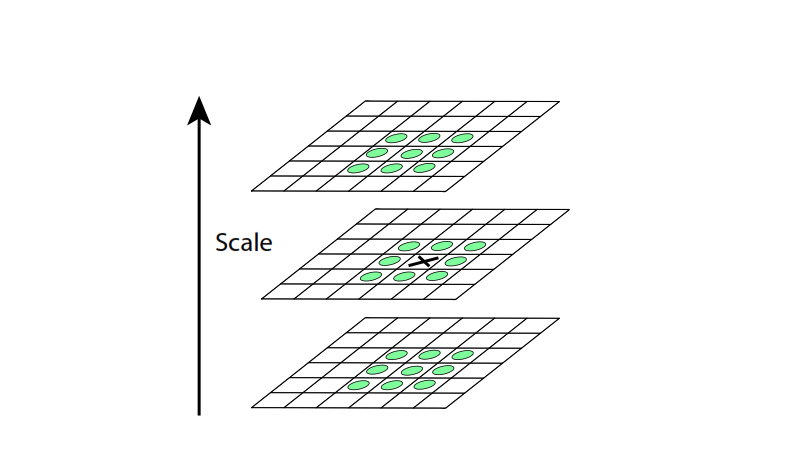
\includegraphics[width=1.0\textwidth]{img/sift2.PNG}
\caption{ Detection of axima and minima of the difference-of-Gaussian .}
\label{fig:sift2}
\end{figure}

This shows that when the difference-of-Gaussian function has scales differing by a constant
factor it already incorporates the  $\sigma ^2 $
scale normalization required for the Laplacian. \\The
factor (k-1) in the equation is a constant over all scales and therefore does not influence
peak location. The approximation error will go to zero as k goes 1, but in practice we have
found that the approximation has almost no impact on the stability of peak detection or
localization for even significant differences in scale, such as $k= \sqrt{2}$
An efficient approach to construction of D(x; y;$\sigma$) is shown in Figure \ref{fig:sift1}. The input image
is incrementally convolved with Gaussians to produce images separated by a constant
factor k in scale space, shown stacked in the left column. \\We choose to divide each octave
of scale space (i.e., doubling of $\sigma$) into an integer number, s, of intervals, so $k = 2^{1/\mathbf{s}}$
Adjacent image scales are subtracted to produce the difference-of-Gaussian images shown
on the right. Once a complete octave has been processed, we resample the Gaussian image
that has twice the initial value of $\sigma$ by taking every second pixel in each row and column. \newline
\newline
The accuracy of sampling relative to $\sigma$ is no different than for the previous octave, while
computation is greatly reduced.

\textbf{Summary of the section :}

In the first step of SIFT, it generates several octaves of the original image. Each octave's image size is half the previous one. Within an octave, images are progressively blurred using the Gaussian Blur operator.
next we use all these octaves to generate Difference of Gaussian images ( Dog ) Two consecutive images in an octave are picked and one is subtracted from the other. Then the next consecutive pair is taken, and the process repeats. This is done for all octaves. The resulting images are an approximation of scale invariant laplacian of gaussian which is good for detecting keypoints .


\subsection{Keypoint localization :}
We wish to identify locations in image scale space that are
invariant with respect to image translation, scaling, and rotation,
and are minimally affected by noise and small distortions.\\
Lindeberg \cite{e} has shown that under some rather
general assumptions on scale invariance, the Gaussian kernel
and its derivatives are the only possible smoothing kernels
for scale space analysis.\\
To achieve rotation invariance and a high level of efficiency,
we have chosen to select key locations at maxima
and minima of a difference of Gaussian function applied in
scale space. This can be computed very efficiently by building
an image pyramid with resampling between each level.
Furthermore, it locates key points at regions and scales of
high variation, making these locations particularly stable for
characterizing the image.\\ Crowley and Parker \cite{f} and Lindeberg
\cite{e} have previously used the difference-of-Gaussian in
scale space for other purposes. In the following, we describe
a particularly efficient and stable method to detect and characterize
the maxima and minima of this function.\\
As the 2D Gaussian function is separable, its convolution
with the input image can be efficiently computed by applying
two passes of the 1D Gaussian function in the horizontal
and vertical directions:

\begin{align}
     g(x)  =\frac{1}{\sqrt{2\pi}\sigma} e^\frac{x^2}{2\sigma^2}
\end{align}


For key localization, all smoothing operations are done using
$\sigma = \sqrt{2}$ , which can be approximated with sufficient accuracy
using a 1D kernel with 7 sample points.\\
The input image is first convolved with the Gaussian
function using $\sigma = \sqrt{2}$ to give an image \textit{A}. This is then
repeated a second time with a further incremental smoothing
of $\sigma = \sqrt{2}$ to give a new image, \textit{B}, which now has an
effective smoothing of $\sigma$ =2. The difference of Gaussian
function is obtained by subtracting image B from A, resulting
in a ratio of $2/\sqrt{2}$ = $ \sqrt{2}$ between the two Gaussians.\\
To generate the next pyramid level, we resample the already smoothed image B using bilinear interpolation with a
pixel spacing of 1.5 in each direction.\\ While it may seem
more natural to resample with a relative scale of$\sqrt{2}$,the
only constraint is that sampling be frequent enough to detect
peaks.\\ The 1.5 spacing means that each newsample will
be a constant linear combination of 4 adjacent pixels. This
is efficient to compute and minimizes aliasing artifacts that
would arise from changing the resampling coefficients.\\
Maxima and minima of this scalespace function are determined
by comparing each pixel in the pyramid to its
neighbours. First, a pixel is compared to its 8 neighbours at
the same level of the pyramid.\\ If it is a maxima or minima
at this level, then the closest pixel location is calculated at
the next lowest level of the pyramid, taking account of the
1.5 times resampling. If the pixel remains higher (or lower)
than this closest pixel and its 8 neighbours, then the test is
repeated for the level above. Since most pixels will be eliminated
within a few comparisons, the cost of this detection is
small and much lower than that of building the pyramid.\\
If the first level of the pyramid is sampled at the same rate
as the input image, the highest spatial frequencies will be ignored.
This is due to the initial smoothing, which is needed
to provide separation of peaks for robust detection. Therefore,
we expand the input image by a factor of 2, using bilinear
interpolation, prior to building the pyramid. This gives
on the order of 1000 key points for a typical
512$\times$512 pixel
image, compared to only a quarter as many without the initial
expansion.

\textbf{Summary of this section :}

Here, we detected the maxima and minima in the DoG images generated in the previous step. This is done by comparing neighbouring pixels in the current scale, the scale "above" and the scale "below".


\subsection{Orientation assignment :}
By assigning a consistent orientation to each keypoint based on local image properties,
the keypoint descriptor can be represented relative to this orientation and therefore achieve
invariance to image rotation.\\ This approach contrasts with the orientation invariant descriptors
of Schmid and Mohr (1997), in which each image property is based on a rotationally
invariant measure.\\ The disadvantage of that approach is that it limits the descriptors that
can be used and discards image information by not requiring all measures to be based on a
consistent rotation.\\

Following experimentation with a number of approaches to assigning a local orientation,
the following approach was found to give the most stable results. The scale of the
keypoint is used to select the Gaussian smoothed image, L, with the closest scale, as all
computations must be performed in a scale invariant manner. For each image sample, $L_{x,y}$ ,the gradient magnitude, m, and orientation, $\theta$, is precomputed using pixel differences:

\begin{align}
 m  =\sqrt{(L_{x+1,y} - L_{x-1,y})^2 + (L_{x,y+1} - L_{x,y-1})^2}
\end{align}
\begin{align}
  \theta = \tan^{\small{-1}}\frac{(L_{x,y+1} - L_{x,y-1})}{(L_{x+1,y} - L_{x-1,y})}
\end{align}

An orientation histogram is formed from the gradient orientations at all sample points
within a circular window around the keypoint. Each sample added to the histogram is
weighted by its gradient magnitude and by a Gaussian-weighted circular window with a $\sigma$
three times that of the scale of the keypoint. The orientation histogram has 36 bins covering
the 360 degree range of orientations.
Peaks in the orientation histogram correspond to dominant directions of local gradients.
The highest local peak in the histogram is detected, and then any other local peak that is
within 80\% of the highest peak is used to also create a keypoint with that orientation.
Therefore, for locations with multiple peaks of similar magnitude, there will be multiple
keypoints created at the same location and scale but different orientations. Only about
15\% of points are assigned multiple orientations, but these contribute significantly to the
stability of matching. Finally, a parabola is fit to the 3 histogram values around each peak
to interpolate the peak position for better accuracy.


\textbf{summary of the section :}

To assign an orientation we use a histogram and a small region around it. Using the histogram, the most prominent gradient orientation(s) are identified. If there is only one peak, it is assigned to the keypoint. If there are multiple peaks above the 80\% mark, they are all converted into a new keypoint (with their respective orientations).

\subsection{Keypoint descriptor :}

Figure \ref{fig:sift4} illustrates the computation of the keypoint descriptor. First the image gradient
magnitudes and orientations are sampled around a keypoint, using the scale of the keypoint
to select the level of Gaussian blur for the image. For efficiency, the gradients are precomputed
for all levels of the pyramid as described in Section 4.1.3 . These are illustrated with
small arrows at each sample location on the left side of Figure \ref{fig:sift4}

\begin{figure}[H]
\centering
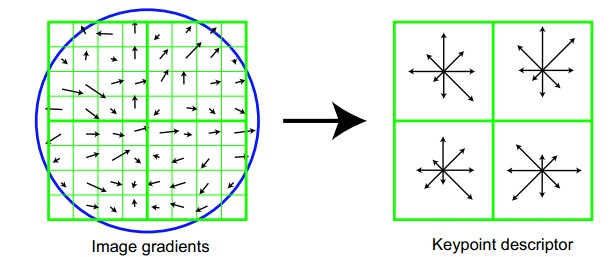
\includegraphics[width=0.8\textwidth]{img/sift4.jpg}
\caption{ Keypoint descriptor }
\label{fig:sift4}
\end{figure}

A Gaussian weighting function with $\sigma$ equal to one half the width of the descriptor
window is used to assign a weight to the magnitude of each sample point. This is illustrated
with a circular window on the left side of Figure \ref{fig:sift4}, although, of course, the weight falls off smoothly. The purpose of this Gaussian window is to avoid sudden changes in the
descriptor with small changes in the position of the window, and to give less emphasis
to gradients that are far from the center of the descriptor, as these are most affected by
misregistration errors.
The keypoint descriptor is shown on the right side of Figure \ref{fig:sift4}. It allows for significant
shift in gradient positions by creating orientation histograms over 4$\times$4 sample regions. The
figure shows eight directions for each orientation histogram, with the length of each arrow
corresponding to the magnitude of that histogram entry. A gradient sample on the left can
shift up to 4 sample positions while still contributing to the same histogram on the right,
thereby achieving the objective of allowing for wider local positional shifts.
It is important to avoid all boundary affects in which the descriptor abruptly changes as
a sample shifts smoothly from being within one histogram to another or from one orientation
to another. Therefore, linear interpolation is used to assign a weight to each histogram
entry according to the distance of the sample from its central value, and the gradient magnitude
of a sample is distributed into the histogram accumulators according to these weights.
The descriptor is formed from a vector containing the values of all the orientation histogram
entries, corresponding to the lengths of the arrows on the right side of Figure \ref{fig:sift4}. The
figure shows a 2$\times$2 array of orientation histograms, whereas our experiments below show
that best results are achieved with a 4$\times$4 array of histograms with 8 orientation bins in each.
Therefore, the experiments in this paper use a 4$\times$4$\times$8 = 128 element feature vector for each
keypoint.
Finally, the feature vector is normalized to reduce the effects of illumination change.
First, the vector is normalized to unit length. A change in image contrast in which each
pixel value is multiplied by a constant will multiply gradients by the same constant, so this
contrast change will be cancelled by vector normalization. A brightness change in which a
constant is added to each image pixel will not affect the gradient values, as they are computed
from pixel differences. However, non linear illumination changes can also occur due
to camera saturation or illumination changes that affect surfaces with different orientations
by differing amounts. These effects can cause a large change in relative magnitudes for
some gradients, but are less likely to affect the gradient orientations. Therefore, we reduce
the influence of gradient magnitudes by thresholding the values in the unit feature vector to
each be no larger than 0.2, and then renormalizing to unit length. This means that matching
the magnitudes for large gradients is no longer as important, and that the distribution of
orientations has greater emphasis. The value of 0.2 was determined experimentally using
differing illuminations for the same objects\\

\textbf{Summary of the section }

Sift take  a 16x16 window of "in-between" pixels around the keypoint. split that window into sixteen 4x4 windows. From each 4x4 window it generate a histogram of 8 bins. Each bin corresponding to 0-44 degrees, 45-89 degrees. Gradient orientations from the 4x4 are put into these bins. This is done for all 4x4 blocks. Finally, it normalize the 128 values .

\subsection{Speeded Up Robust Features (SURF) :}
SURF (Speeded Up Robust Features), is a feature detector, we talked about SIFT before, and SURF is sort of derivative of SIFT. SURF is based on sums of 2D Haar wavelet responses and makes an efficient use of integral images.

we will not go through  the whole literature  of SURF, because its idea is very similar to SIFT, so we will only talk about \textbf{the difference between these two methods}.

\subsection{ABOUT HESSIAN}
In Sift method, we use Difference of Gaussian (DoG) to build the image pyramid, and in Surf, we simply use an integer approximation to the determinant of Hessian blob detector .

Given a pixel, the Hessian of this pixel is something like:
$\sigma^2\nabla^2G$ \\

\begin{gather}
H(f(x,y)) =
\begin{bmatrix}
                 {\frac {\partial^2 f} {\partial x^2}} && { \frac {\partial^2 f} {\partial x.\partial y} }\\
                 {\frac  {\partial^2 f}{\partial x.\partial y}} && { \frac {\partial^2 f} {\partial y^2}}
\end{bmatrix}
\end{gather}

For adapt to any scale, we filtered the image by a Gaussian kernel, so given a point X = (x, y), the Hessian matrix H(x,$\sigma$) in x at scale $\sigma$ is defined as:
\begin{gather}
 \mathcal{H}(x,\sigma) =
\begin{bmatrix}
                 {L_{xx}(x,\sigma)}  && {L_{xy}(x,\sigma)} \\
                 {L_{xy}(x,\sigma)} && {L_{yy}(x,\sigma)}
\end{bmatrix}
\end{gather}
where ${L_{xx}(x,\sigma)}$ is the convolution of the Gaussian second order derivative with the image I in point x, and similarly for ${L_{xy}(x,\sigma)}$ and ${L_{yy}(x,\sigma)}$.\\
First convolution, then second order derivative, we now approximate these two processes with one single filter.\\


\begin{figure}[H]
\centering
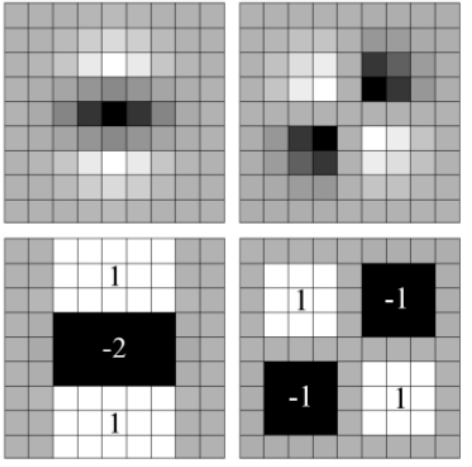
\includegraphics[width=0.55\textwidth]{img/surf4.PNG}
\caption{${L_{yy}(x,\sigma)}$ and${L_{xy}(x,\sigma)}$ Discretized
Gaussians and the approximations $D_{yy}$ and $D_{xy}$}
\label{fig:surf1}
\end{figure}

These approximate second order Gaussian derivatives and can be evaluated at a very low computational cost using integral images, and this is part of the reason why SURF is fast.

Now we can represent the determinant of the Hessian (approximated) as:

\begin{figure}[H]
\centering
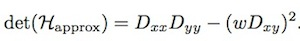
\includegraphics[width= 0.4\textwidth]{img/det.jpeg}

\label{fig:surfdet}
\end{figure}
and we can use 0.9 for w by Bay’s suggestion.

\subsection{ABOUT PYRAMID :}

In Sift, we use DOG to build image pyramids, the pyramid have several octaves, and there are several images layers in each octave. The difference between Sift pyramid and Surf pyramid is, in Sift, we use different scales of image; and in Surf, we use different scales of Gaussian masks, while the scale of image is always unaltered. By this, we save a lot of time by not downsampling image.

\begin{figure}[H]
\centering
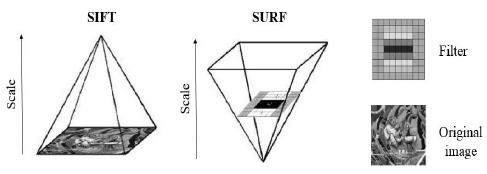
\includegraphics[width=0.6\textwidth]{img/surf2.png}
\caption{Where SIFT(left) downscales the image,
SURF(right) uses larger and larger filters}
\label{fig:surf2}
\end{figure}

 Instead of iteratively reducing the image size (left), the use of integral images allows the upscaling of the filter at constant cost (right).\\
 
 \subsection{ABOUT FEATURE DESCRIPTOR}
 In Sift, we use an orientation histogram, and find the largest orientation value and also those values that are over 80\% of the largest, and use these orientations as the main orientation of the feature descriptor. In Surf, we use the sum of the Haar wavelet response around the point of interest.

\begin{figure}[H]
\centering
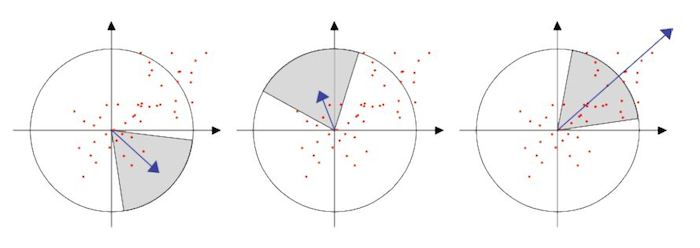
\includegraphics[width=0.6\textwidth]{img/surf3.jpg}
\caption{descriptor computation }
\label{fig:surf3}
\end{figure}

We first calculate the Haar wavelet responses in x and y direction within a circular neighborhood of radius 6s around the interest point, with s the scale at which the interest point was detected. We calculate the sum of vertical and horizontal wavelet responses in a scanning aria, then change the scanning orientation (add $\pi$/3), and recalculate, until we find the orientation with largest sum value, this orientation is the main orientation of feature descriptor.

Now it’s time to extract the descriptor. First we construct a square region centered around the feature point, and oriented along the main orientation we already got above, the size of this window is 20s,s is the scale at which the interest point was detected. Second we split this region up regularly into smaller 4$\times$4 square subregions, for each subregion, we compute Haar wavelet responses at 5$\times$5 regularly spaced sample points.


\begin{figure}[H]
\centering
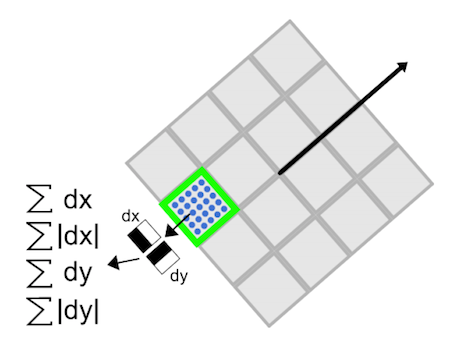
\includegraphics[width=0.5\textwidth]{img/surf5.png}
\caption{computation of dx and dy of Haar  }
\label{fig:surf5}
\end{figure}

We extract the sum of values of the responses in both x and y orientation, furthermore, we extract the sum of the absolute values of the responses, hence, each subregion has a 4-D descriptor vector v. Concatenating this for all 4$\times$4 subregions, our final descriptor is a 64-D vector. (In Sift, our descriptor is 128-D vector, so this is part of the reason that SURF is faster than Sift.)\\


\section{Differences and Preference :}
The two main advantages of SURF over SIFT is that SURF uses Laplacian of Gaussian so as to have a distinction
between background and foreground features, and secondly, SURF uses only 64 dimensional vector compared to 128 dimensional vector for SIFT . This helps in fast feature computation and also the quick matching capability.
The two different steps used by SURF to determine the local descriptor vectors are A. Keypoint Detection B. Keypoint Descriptor, which were  explained above \ref{} and \ref{}.

This makes Surf as our best candidate for gesture recognition  since it offers high number of stable features against Scale invariance and rotation invariance , of course lesser than Sift but it does not worth the Computational operations of up scaling pyramid used in sift Nor the \textbf{valuable }time consumed .

later on we will Experimentally demonstrate that Surf achieved  better accuracy than sift in Hand gesture Recognition  . However Even if Surf is less expensive than sift but still computationally expensive which is bad for our purposes ,Since what describe a Good HGR is its ability to interpret  and interact with the Signer performer in real time , That's where Fouriere descriptor Appears to give accurate and a Very Fast feature extractor which will meet our requirement for a robust and Real time application  .


\section{Fourier Shape Descriptor } \label{FDT}
The Fourier transformed coefficients from the Fourier
Descriptors of the shape represent the shape of the object in
the frequency domain. The general features of the shape can
be found in the lower frequency descriptors, while the higher
frequency descriptors contain information about the shape
details \cite{20}
Before applying Fourier transform on the shape boundary, it
is first normalized for matching purposes; this is done by
sampling the boundary of each shape to have the same number
of data points. The larger the number of sampled points the
more details in the representation of the shape this results in
more accurate matching. While a smaller number of sampled
points reduce the accuracy of the matching results but on the
other hand it will improve the computational efficiency. \\

After normalization we to apply Fourier transform to the
shape signature. A shape signature is any 1-D function
representing 2-D areas or boundaries. The shape signature we
used is complex coordinates. A complex coordinates function
is the complex form of the boundary coordinates \cite{20}. \\
\begin{gather}
    z_{i} = x_{i}+j y_{i} , i\in [1,N]
\end{gather}\\
For each shape we select N points with equal point
sampling. In order to facilitate the use of Fast Fourier
Transform (FFT), the number of sampled points is chosen to
be power of two. Assuming the number of sampled points is
N the Fourier transform gives N Fourier coefficients Cl. The
coefficients are usually called Fourier descriptors of the shape. 
\begin{gather}
C_{l}= \sum_{i=0}^{N-1} z_{i}e{\frac{-j 2\pi il}{N}} , l = 0,...,N-1
\end{gather}
The magnitude of the Fourier
Transform of this set forms a unique shape signature, which can be used for generalized
gesture classification.
In addition, this descriptor is rotationally invariant. Shifts in the silhouette contour
points, which is the cause of rotation, will be appear as phase delays in frequency
domain. However, since only the magnitude of the Fourier coefficients is considered,
the phase (or equivalently, the rotation) is ignored. So, this method is rotationally
invariant while remaining computationally fast\\


\textbf{Generating the Fourier Descriptor: }
\begin{enumerate}
    \item $X_{c} = \frac{1}{N}\sum_{n=0}^{N-1} x(i) , Y_{c} = \frac{1}{N}\sum_{n=0}^{N-1} y(i)  = 1$ , where N is number of hand object pixels 
    \item Take the magnitude of the N point DFT of these points :\\
              \textbf{ abs(FT{r[n]}) = a[m] , for m = 0..N-1 }.
    \item Normalize the Fourier coefficients by the DC value (Scale Invariance) .
    \item Keep the first 7 normalized coefficients (skip DC, which is always 1) .

\end{enumerate}


This is the Fourier Descriptor for a single shape.\\

\textbf{Make a Dictionary : } For a set of images of the same gesture, compute the average Fourier shape descriptor and add it to the dictionary with the same label.  Repeat for all desired gestures.

\textbf{Classification  : }Compute the Fourier descriptor for each new sample.  Compare it with each stored gesture in the dictionary using  Euclidean distance measure.  The label of the minimum distance is the desired gesture( Nearest Neighbor happens to be the most efficient method of classification )

\subsection{Covariance Matrix Approach :}
This approach \cite{21}
performs human action recognition by looking at a sequence of whole body silhouettes
over time, a silhouette tunnel, captured by the Kinect. A 13 dimensional feature vector
is defined, where 3 values are row, column, and time, 8 values are based on the shape of
the silhouette, and the last 2 are a measure of the temporal similarity.
However, this feature vector is general enough to work with hand silhouettes in addition
to full bodies. So, it is possible to modify the shape feature vector to work with static
hand gestures by reducing the dimensionality. This can be accomplished by removing
the time dependence and temporal similarity terms. The result is a generalized 10
dimensional feature vector applicable to static shape recognition.\\

\textbf{Create the Feature Vector :}\\
\begin{enumerate}
    \item Compute the 10-dimensional feature vector adapted from Guo \cite{21} : 
    
    \item f(x,y) = [x,y,de,dw,dn,ds,dne,dse,dnw]
    \begin{itemize}
        \item x = col , y=row
        \item d =  Euclidean distance from (x,y) to the nearest boundary point in the specified
direction \\
east, west, north, south, northeast, southwest, southeast, northwest
    \end{itemize}
    \item Scale Invariance 
    \begin{itemize}
        \item Divide each spatial feature by the square root of the silhouette area
     
    \end{itemize}
    \item Compute the Covariance Matrix: 
    \begin{itemize}
        \item $cov(f(\textbf{S}))=\frac{1}{|S|}\sum_{(x,y) \in S }(f(x,y)-\mu_{F})(f(x,y)-\mu_{F})^{T}$
        \item \textbf{S} = area of silhouettte 
        \item $\mu_{F} = \frac{1}{|S|}\sum_{(x,y) \in S } f(x,y) $
    \end{itemize}
    
\end{enumerate}
\textbf{Build a Dictionary }\\
For a set of images of the same gesture, compute the Covariance Matrix and add it to
the dictionary with the same label. Repeat for all desired gestures.\\
\textbf{Classification }\\
As noted in Guo \cite{21}, the set of all covariance matrices lie on a Riemannian
manifold. So, a Euclidean distance measure cannot be used. Instead, the distance
between two covariance matrices on this manifold is defined as:\\
$$d(C,C') = \sqrt{\sum_{k=1}^{10} (\ln \lambda_{k}(C,C'))^{2}}$$ \\
\texttt{where $\lambda_{k}(C,C')$ are generalized eigenvalues of C and C'\\
C = convariance Matrix of new sample ,  C' = Reference from dictionary  } \\

The label of the minimum distance gesture is used for classification .

\begin{table}[!h]
\centering
\caption{Pros and Con of Covariance approach }
\label{my-label}
\begin{tabular}{lllll}
\cline{1-2}
\multicolumn{1}{|l|}{\textbf{\begin{tabular}[c]{@{}l@{}}Pros:\\  1. Complex Gesture .\\  2. High accuracy.\\  3. Scale invariant.\end{tabular}}} & \multicolumn{1}{l|}{\textbf{\begin{tabular}[c]{@{}l@{}}Con :\\ 1. Not rotation Invariant . \\           \\        \\ \end{tabular}}} &  &  &  \\ \cline{1-2}
                                                                                                                                                 &                                                                                                           &  &  &  \\
                                                                                                                                                 &                                                                                                           &  &  &  \\
                                                                                                                                                 &                                                                                                           &  &  & 
\end{tabular}
\end{table}

\newpage
 
 \section{ Conclusion : }
 in this chapter we went through Two types of descriptors :\\
\textbf{the first} are  Local descriptors SIFT and SURF  descriptors that typically involves more intense computations and algorithms, often requiring floating point
calculations, and may consume considerable memory.but generally they give a high  accuracy Additionally to their stable performance even against scale variation and Rotation variation too , the following table is summarizing the Differences of these two descriptors :

\begin{table}[!h]
\centering
\caption{COMPARISON OF SIFT AND SURF}
\label{surfvssift}
\begin{tabular}{l|l|l|ll}
\cline{2-3}
\textbf{}                                                                                     & \textbf{SIFT}                                                                                                                                                     & \textbf{SURF}                                                                                                                             &  &  \\ \cline{1-3}
\multicolumn{1}{|l|}{\textbf{\begin{tabular}[c]{@{}l@{}}Keypoint\\ Detection\end{tabular}}}   & \textbf{\begin{tabular}[c]{@{}l@{}}Different scale image\\ convoluted with\\ Gaussian function\end{tabular}}                                                      & \textbf{\begin{tabular}[c]{@{}l@{}}Original Image is\\ convoluted with\\ Different scale box\\ filter\end{tabular}}                       &  &  \\ \cline{1-3}
\multicolumn{1}{|l|}{\textbf{\begin{tabular}[c]{@{}l@{}}Keypoint\\ Description\end{tabular}}} & \textbf{\begin{tabular}[c]{@{}l@{}}Gradient amplitude of\\ a square area is\\ calculated with\\ maximum gradient\\ strength as the main\\ direction\end{tabular}} & \textbf{\begin{tabular}[c]{@{}l@{}}A Haar Wavelet response\\  is used to\\ calculate \\ each sector in\\ a \\ circular area\end{tabular}} &  &  \\ \cline{1-3}
\multicolumn{1}{|l|}{\textbf{Dimensions}}                                                     & 128                                                                                                                                                               & 64                                                                                                                                        &  &  \\ \cline{1-3}
\end{tabular}
\end{table}



\textbf{The second } are Basis Space descriptors   , A basis space is composed of a set of functions, the basis functions, which are
composed together as a set, such as a series like the Fourier series and covariance Matrix  . \\
Fourier descriptors represent feature data as sine and cosine terms, which can be
observed in a Fourier Power Spectrum. The Fourier series, Fourier transform, and Fast
Fourier transform are used for a wide range of signal analysis, including 1D, 2D, and 3D
problems. No discussion of image processing or computer vision is complete without
Fourier methods .

With this summary we are done from Feature detection / extraction and we will move on to the next Phase of building  our HGR System , which is  Feature classification using Machine learning algorithms that's going to be the goal of next section .

\chapter{Descriptors}

\section{introduction}

Over the last decades, image feature detectors and descriptors have become popular tools in the computer vision community and they are being applied widely in a large number of applications. Image representation , image classification and retrieval  , object recognition and matching  3D scene reconstruction , motion tracking   texture classification , robot localization, all rely on the presence of stable and representative features in the image. Thus, detecting and extracting the image features are vital steps for these applications.
Hence The need for a Descriptor that can detect and extract Features 
and Since our HGR system needs a Features detector that can be stable in most cases which will  full fill our need to Recognize the Gesture performed by the user .\\

\textit{Note : The Definition of SIFT  Descriptor might be long and has a lot of Definitions because Sift is considered as the most  powerful and widely used local descriptor in object recognition and image classification Hence the Literature focus on it  , and as a guarantee  to ensure the understanding of  Sift definition and key words  we will summarize all Sift's  Definition  IN THE END OF EVERY SECTION }

\section{Definitions and Principles:}

\subsection{Global and Local Features}
the following definition was given by M. Hassaballah et al in \ref{}. 
In the global feature representation, the image is represented by one multidimensional
feature vector, describing the information in the whole image.\\
In other words, the global representation method produces a single vector with values that
measure various aspects of the image such as color, texture or shape. Practically, a
single vector from each image is extracted and then two images can be compared by
comparing their feature vectors.\\ For example, when one wants to distinguish images
of a sea (blue) and a forest (green), a global descriptor of color would produce quite
different vectors for each category. In this context, global features can be interpreted
as a particular property of image involving all pixels.
This property can be color
histograms, texture, edges or even a specific descriptor extracted from some filters
applied to the image \cite{h}.\\ On the other hand, the main goal of local feature representation
is to distinctively represent the image based on some salient regions while
remaining invariant to viewpoint and illumination changes. Thus, the image is represented
based on its local structures by a set of local feature descriptors extracted
from a set of image regions called interest regions (i.e., keypoints) as illustrated in
Fig.\ref{fig:Ft1} Most local features represent texture within the image patch.

\begin{figure}[H]
\centering
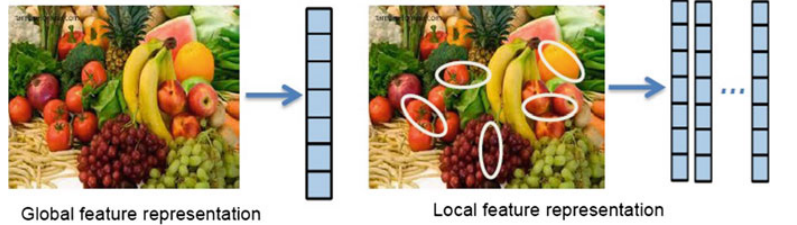
\includegraphics[width=0.9\textwidth]{img/features.PNG}
\caption{ Global and local image features representation }
\label{fig:Ft1}
\end{figure}

Generally, using what kind of features might greatly depend on the applications
on hand. Developers prefer the most discriminative ones. For example, a person with
a bigger nose and smaller eyes, and a person with a smaller nose and bigger eyes
may have similar mug shot in terms of histogram or intensity distribution. Then, local
features or the global pattern distilled from local feature clusters seem to be more
discriminative. Whereas, for very large datasets in the web scale image indexing
application, it is appropriate to consider global features. Also, global features are
useful in applications where a rough segmentation of the object of interest is available.
The advantages of global features are that they are much faster and compact
while easy to compute and generally require small amounts of memory.\\ Nevertheless,
the global representation suffers from well known limitations, in particular they
are not invariant to significant transformations and sensitive to clutter and occlusion.\\In some applications, such as copy detection, most of the illegal copies are very  similar to the original; they have only suffered from compression, scaling or limited
cropping. In contrast, the advantage of local features is their superior performance \cite{i}. Meanwhile, using local features for large scale image search have much higher performance than global features provide \cite{k}.\\ Besides, as the local structures are more distinctive and stable than other structures in smooth regions, it is expected to be more useful for image matching and object recognition.\\ However, they usually require a significant amount of memory because the image may have hundreds of local features.\\ As a solution for this problem, researchers suggest aggregating local image descriptors into a very compact vector representation and optimizing the
dimensionality reduction of these vectors \cite{k}


\subsection{Characteristics of Feature Detectors}

Tuytelaars and Mikolajczyk \cite{MM} define a local feature as \textit{ “it is an image pattern
which differs from its immediate neighborhood”.} Thus, they consider the purpose of
local invariant features is to provide a representation that allows to efficiently match
local structures between images. That is, we want to obtain a sparse set of local
measurements that capture the essence of the underlying input images and encode
their interesting structures. To meet this goal, the feature detectors and extractors
must have certain properties keeping in mind that the importance of these properties
depends on the actual application settings and compromises need to be made. The
following properties are important for utilizing a feature detector in computer vision
applications:
\begin{itemize}
\item Robustness, the feature detection algorithm should be able to detect the same feature
locations independent of scaling, rotation, shifting, photometric deformations,
compression artifacts, and noise
\item Repeatability, the feature detection algorithm should be able to detect the same
features of the same scene or object repeatedly under variety of viewing conditions.
\item Accuracy, the feature detection algorithm should accurately localize the image
features (same pixel locations), especially for image matching tasks, where precise
correspondences are needed to estimate the epipolar geometry.
\item Generality, the feature detection algorithm should be able to detect features that
can be used in different applications.
\item Efficiency, the feature detection algorithm should be able to detect features in new
images quickly to support real time applications.
\item Quantity, the feature detection algorithm should be able to detect all or most of the
features in the image. Where, the density of detected features should reflect the
information content of the image for providing a compact image representation.
\end{itemize}

\textbf{in this project We are going to use Local Features( descriptors) For its Efficiency and scale , Rotation  Invariant }\\
\section{Spectra descriptors :}
\subsection{SIFT - Scale Invariant Feature Transforms} \label{siftSection}

The Scale Invariant Feature Transform (SIFT) developed by Lowe \ref{} is the most well known method for finding interest points and feature descriptors, providing invariance to scale, rotation, illumination, affine distortion, perspective and similarity
transforms, and noise. Lowe demonstrates that by using several SIFT descriptors together to describe an object, there is additional invariance to occlusion and clutter. We provide some detail here on SIFT since it is well designed and well known.


\begin{enumerate}
\item Scale-Space Extrema Detection :
The first stage of computation must search over all
scales and image locations, but it can be implemented efficiently by using a difference of-Gaussian
function to identify potential interest points that are invariant to scale and
orientation.
\item Keypoint localization :
At each candidate location, a detailed model is fit to determine
location, scale, and contrast. Keypoints are selected based on measures of their
stability.
\item Orientation assignment :
One or more orientations are assigned to each keypoint
location based on local image properties. All future operations are performed relative
to the assigned orientation, scale, and location for each feature, providing invariance
to these transformations.
\item Keypoint descriptor  :
The local image gradients are measured at the selected scale
in the region around each keypoint, and transformed into a representation that allows
for local shape distortion and change in illumination.
\end{enumerate}

An important aspect of this approach is that it generates large numbers of features that
densely cover the image over the full range of scales and locations.\\ A typical image of size
500$\times$500 pixels will give rise to about 2000 stable features (although this number depends
on both image content and choices for various parameters).\\ The quantity of features is
particularly important for object recognition, where the ability to detect small objects in
cluttered backgrounds requires that at least 3 to 6 features be correctly matched from each
object for reliable identification.
For image matching and recognition, features are first extracted from a set of reference
images and stored in a database.\\ A new image is matched by individually comparing
each feature from the new image to this previous database and finding candidate matching
features based on Euclidean distance of their feature vectors.\\
The keypoint descriptors are highly distinctive, which allows a single feature to find its
correct match with good probability in a large database of features. 



\subsection{Scale-Space Extrema Detection :}
As described in [\ref{siftSection}], we will detect keypoints using a sequential filtering approach
that uses efficient algorithms to identify candidate locations that are then examined
in further detail.\\ The first stage of keypoint detection is to identify locations and scales that
can be repeatably assigned under differing views of the same object. Detecting locations
that are invariant to scale change of the image requires that we search for stable features
across all possible changes of scale, using a continuous function of scale known as scale
space (Witkin, 1983).\\
It has been shown by Koenderink (1984) and Lindeberg (1994) that under a variety of reasonable assumptions the only possible scale space kernel is the Gaussian function.
Therefore, the scale space of an image is defined as a function, L(x, y, $\sigma$), that is produced
from the convolution of a variable scale Gaussian, G(x, y,$\sigma$), with an input image, I(x, y):\\

L(x, y, $\sigma$) = G(x, y,$\sigma$) * I(x, y),


where * is the convolution operation in x and y, and

\begin{align*} 
 G(x, y,\sigma )  =\frac{1}{2\pi\sigma^2} e^\frac{-( x^2 -  y^2)}{2\sigma^2}  
\end{align*}

To efficiently detect stable keypoint locations in scale space, we have proposed (Lowe,
1999) using scale space peaks in the difference-of-Gaussian function convolved with the
image, D(x, y, $\sigma$), which can be computed from the difference of two nearby scales separated
by a constant factor k:
\begin{align}
D(x, y, \sigma) &= (G(x, y, k\sigma) - G(x, y,\sigma) * I(x, y)\\
                 &= L(x, y, k\sigma) - L(x, y, \sigma) .
   \end{align}               
                  
There are a number of reasons for choosing this function. First, it is a particularly
efficient function to compute, as the smoothed images, L  need to be computed in any
case for scale space feature description, and D can therefore be computed by simple image
subtraction.

\begin{figure}[H]
\centering
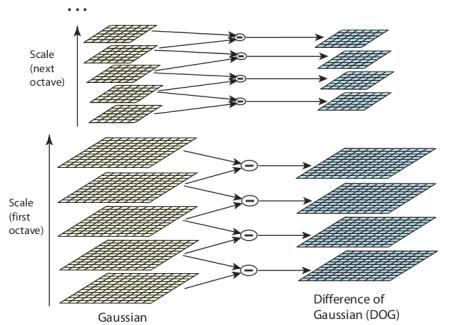
\includegraphics[width=0.8\textwidth]{img/sift_dog.jpg}
\caption{ For each octave of scale space, the initial image is repeatedly convolved with Gaussians to
produce the set of scale space images shown on the left. Adjacent Gaussian images are subtracted
to produce the difference-of-Gaussian images on the right. After each octave, the Gaussian image
is down sampled by a factor of 2, and the process repeated.}
\label{fig:sift1}
\end{figure}

In addition, the difference-of-Gaussian function provides a close approximation to the
scale normalized Laplacian of Gaussian, $\sigma^2\nabla^2 G $
, as studied by Lindeberg (1994).\\Lindeberg
showed that the normalization of the Laplacian with the factor $\sigma^2$
is required for true scale invariance. In detailed experimental comparisons, Mikolajczyk (2002) found that the maxima and minima of $\sigma^2\nabla^2 G $  produce the most stable image features compared to a range
of other possible image functions, such as the gradient, Hessian, or Harris corner function.\\
The relationship between D and $\sigma^2\nabla^2G $
G can be understood from the heat diffusion
equation (parameterized in terms of $\sigma$ rather than the more usual t = $\sigma^2$):\\

\begin{align}
    \frac {\partial G} {\partial \sigma} = \sigma \nabla^2 G 
\end{align}




From this, we see that$\nabla^2$ G can be computed from the finite difference approximation to  $\frac{\partial G}{\partial \sigma }$ , using the difference of nearby scales at k$\sigma$ and $\sigma$ :\\


\begin{align}
      \sigma \nabla^2 G =   \frac {\partial G} {\partial \sigma} \approx   \frac {G(x,y,k \sigma) -  G(x,y,\sigma)}{ k \sigma - \sigma}  
\end{align}


and therefore,


\begin{align}
      G(x,y,k \sigma) -  G(x,y,\sigma)  \approx (k - 1)  \sigma^2\nabla^2G 
\end{align}

\begin{figure}[H]
\centering
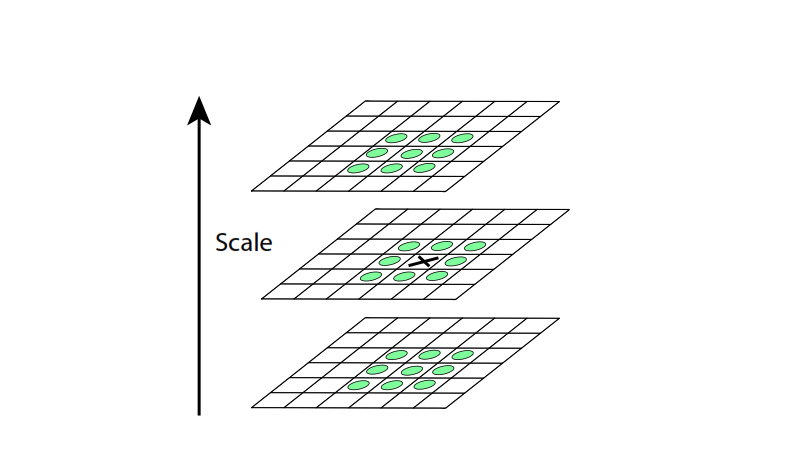
\includegraphics[width=1.0\textwidth]{img/sift2.PNG}
\caption{ Maxima and minima of the difference-of-Gaussian images are detected by comparing a
pixel (marked with X) to its 26 neighbors in 3x3 regions at the current and adjacent scales (marked
with circles).}
\label{fig:sift2}
\end{figure}

This shows that when the difference-of-Gaussian function has scales differing by a constant
factor it already incorporates the  $\sigma ^2 $
scale normalization required for the Laplacian. \\The
factor (k-1) in the equation is a constant over all scales and therefore does not influence
peak location. The approximation error will go to zero as k goes 1, but in practice we have
found that the approximation has almost no impact on the stability of peak detection or
localization for even significant differences in scale, such as $k= \sqrt{2}$
An efficient approach to construction of D(x; y;$\sigma$) is shown in Figure \ref{fig:sift1}. The input image
is incrementally convolved with Gaussians to produce images separated by a constant
factor k in scale space, shown stacked in the left column. \\We choose to divide each octave
of scale space (i.e., doubling of $\sigma$) into an integer number, s, of intervals, so $k = 2^{1/\mathbf{s}}$
Adjacent image scales are subtracted to produce the difference-of-Gaussian images shown
on the right. Once a complete octave has been processed, we resample the Gaussian image
that has twice the initial value of $\sigma$ by taking every second pixel in each row and column. \newline
\newline
The accuracy of sampling relative to $\sigma$ is no different than for the previous octave, while
computation is greatly reduced.

\textbf{Summary of the section :}

In the first step of SIFT, it generates several octaves of the original image. Each octave's image size is half the previous one. Within an octave, images are progressively blurred using the Gaussian Blur operator.
next we use all these octaves to generate Difference of Gaussian images ( Dog ) Two consecutive images in an octave are picked and one is subtracted from the other. Then the next consecutive pair is taken, and the process repeats. This is done for all octaves. The resulting images are an approximation of scale invariant laplacian of gaussian which is good for detecting keypoints .


\subsection{Keypoint localization :}
We wish to identify locations in image scale space that are
invariant with respect to image translation, scaling, and rotation,
and are minimally affected by noise and small distortions.\\
Lindeberg \cite{e} has shown that under some rather
general assumptions on scale invariance, the Gaussian kernel
and its derivatives are the only possible smoothing kernels
for scale space analysis.\\
To achieve rotation invariance and a high level of efficiency,
we have chosen to select key locations at maxima
and minima of a difference of Gaussian function applied in
scale space. This can be computed very efficiently by building
an image pyramid with resampling between each level.
Furthermore, it locates key points at regions and scales of
high variation, making these locations particularly stable for
characterizing the image.\\ Crowley and Parker \cite{f} and Lindeberg
\cite{e} have previously used the difference-of-Gaussian in
scale space for other purposes. In the following, we describe
a particularly efficient and stable method to detect and characterize
the maxima and minima of this function.\\
As the 2D Gaussian function is separable, its convolution
with the input image can be efficiently computed by applying
two passes of the 1D Gaussian function in the horizontal
and vertical directions:

\begin{align}
     g(x)  =\frac{1}{\sqrt{2\pi}\sigma} e^\frac{x^2}{2\sigma^2}
\end{align}


For key localization, all smoothing operations are done using
$\sigma = \sqrt{2}$ , which can be approximated with sufficient accuracy
using a 1D kernel with 7 sample points.\\
The input image is first convolved with the Gaussian
function using $\sigma = \sqrt{2}$ to give an image \textit{A}. This is then
repeated a second time with a further incremental smoothing
of $\sigma = \sqrt{2}$ to give a new image, \textit{B}, which now has an
effective smoothing of $\sigma$ =2. The difference of Gaussian
function is obtained by subtracting image B from A, resulting
in a ratio of $2/\sqrt{2}$ = $ \sqrt{2}$ between the two Gaussians.\\
To generate the next pyramid level, we resample the already smoothed image B using bilinear interpolation with a
pixel spacing of 1.5 in each direction.\\ While it may seem
more natural to resample with a relative scale of$\sqrt{2}$,the
only constraint is that sampling be frequent enough to detect
peaks.\\ The 1.5 spacing means that each newsample will
be a constant linear combination of 4 adjacent pixels. This
is efficient to compute and minimizes aliasing artifacts that
would arise from changing the resampling coefficients.\\
Maxima and minima of this scalespace function are determined
by comparing each pixel in the pyramid to its
neighbours. First, a pixel is compared to its 8 neighbours at
the same level of the pyramid.\\ If it is a maxima or minima
at this level, then the closest pixel location is calculated at
the next lowest level of the pyramid, taking account of the
1.5 times resampling. If the pixel remains higher (or lower)
than this closest pixel and its 8 neighbours, then the test is
repeated for the level above. Since most pixels will be eliminated
within a few comparisons, the cost of this detection is
small and much lower than that of building the pyramid.\\
If the first level of the pyramid is sampled at the same rate
as the input image, the highest spatial frequencies will be ignored.
This is due to the initial smoothing, which is needed
to provide separation of peaks for robust detection. Therefore,
we expand the input image by a factor of 2, using bilinear
interpolation, prior to building the pyramid. This gives
on the order of 1000 key points for a typical
512$\times$512 pixel
image, compared to only a quarter as many without the initial
expansion.

\textbf{Summary of this section :}

Here, we detected the maxima and minima in the DoG images generated in the previous step. This is done by comparing neighbouring pixels in the current scale, the scale "above" and the scale "below".


\subsection{Orientation assignment :}
By assigning a consistent orientation to each keypoint based on local image properties,
the keypoint descriptor can be represented relative to this orientation and therefore achieve
invariance to image rotation.\\ This approach contrasts with the orientation invariant descriptors
of Schmid and Mohr (1997), in which each image property is based on a rotationally
invariant measure.\\ The disadvantage of that approach is that it limits the descriptors that
can be used and discards image information by not requiring all measures to be based on a
consistent rotation.\\

Following experimentation with a number of approaches to assigning a local orientation,
the following approach was found to give the most stable results. The scale of the
keypoint is used to select the Gaussian smoothed image, L, with the closest scale, as all
computations must be performed in a scale invariant manner. For each image sample, $L_{x,y}$ ,the gradient magnitude, m, and orientation, $\theta$, is precomputed using pixel differences:

\begin{align}
 m  =\sqrt{(L_{x+1,y} - L_{x-1,y})^2 + (L_{x,y+1} - L_{x,y-1})^2}
\end{align}
\begin{align}
  \theta = \tan^{\small{-1}}\frac{(L_{x,y+1} - L_{x,y-1})}{(L_{x+1,y} - L_{x-1,y})}
\end{align}

An orientation histogram is formed from the gradient orientations at all sample points
within a circular window around the keypoint. Each sample added to the histogram is
weighted by its gradient magnitude and by a Gaussian-weighted circular window with a $\sigma$
three times that of the scale of the keypoint. The orientation histogram has 36 bins covering
the 360 degree range of orientations.
Peaks in the orientation histogram correspond to dominant directions of local gradients.
The highest local peak in the histogram is detected, and then any other local peak that is
within 80\% of the highest peak is used to also create a keypoint with that orientation.
Therefore, for locations with multiple peaks of similar magnitude, there will be multiple
keypoints created at the same location and scale but different orientations. Only about
15\% of points are assigned multiple orientations, but these contribute significantly to the
stability of matching. Finally, a parabola is fit to the 3 histogram values around each peak
to interpolate the peak position for better accuracy.


\textbf{summary of the section :}

To assign an orientation we use a histogram and a small region around it. Using the histogram, the most prominent gradient orientation(s) are identified. If there is only one peak, it is assigned to the keypoint. If there are multiple peaks above the 80\% mark, they are all converted into a new keypoint (with their respective orientations).

\subsection{Keypoint descriptor :}

Figure \ref{fig:sift4} illustrates the computation of the keypoint descriptor. First the image gradient
magnitudes and orientations are sampled around a keypoint, using the scale of the keypoint
to select the level of Gaussian blur for the image. For efficiency, the gradients are precomputed
for all levels of the pyramid as described in Section 4.1.3 . These are illustrated with
small arrows at each sample location on the left side of Figure \ref{fig:sift4}

\begin{figure}[H]
\centering
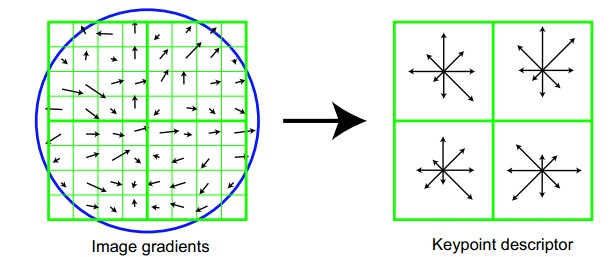
\includegraphics[width=0.8\textwidth]{img/sift4.jpg}
\caption{ A keypoint descriptor is created by first computing the gradient magnitude and orientation
at each image sample point, as shown on the left. These are weighted by a Gaussian window,
indicated by the overlayed circle. These samples are then accumulated into orientation histograms
summarizing the contents over larger regions, as shown on the right, with the length of each arrow
corresponding to the sum of the gradient magnitudes near that direction within the region. To reduce
clutter, this figure shows a 2$\times$2 descriptor array computed from an 8$\times$8 set of samples, whereas most
experiments in this paper use 4x4 descriptors computed from a 16$\times$16 sample array..}
\label{fig:sift4}
\end{figure}

A Gaussian weighting function with $\sigma$ equal to one half the width of the descriptor
window is used to assign a weight to the magnitude of each sample point. This is illustrated
with a circular window on the left side of Figure \ref{fig:sift4}, although, of course, the weight falls off smoothly. The purpose of this Gaussian window is to avoid sudden changes in the
descriptor with small changes in the position of the window, and to give less emphasis
to gradients that are far from the center of the descriptor, as these are most affected by
misregistration errors.
The keypoint descriptor is shown on the right side of Figure \ref{fig:sift4}. It allows for significant
shift in gradient positions by creating orientation histograms over 4$\times$4 sample regions. The
figure shows eight directions for each orientation histogram, with the length of each arrow
corresponding to the magnitude of that histogram entry. A gradient sample on the left can
shift up to 4 sample positions while still contributing to the same histogram on the right,
thereby achieving the objective of allowing for wider local positional shifts.
It is important to avoid all boundary affects in which the descriptor abruptly changes as
a sample shifts smoothly from being within one histogram to another or from one orientation
to another. Therefore, linear interpolation is used to assign a weight to each histogram
entry according to the distance of the sample from its central value, and the gradient magnitude
of a sample is distributed into the histogram accumulators according to these weights.
The descriptor is formed from a vector containing the values of all the orientation histogram
entries, corresponding to the lengths of the arrows on the right side of Figure \ref{fig:sift4}. The
figure shows a 2$\times$2 array of orientation histograms, whereas our experiments below show
that best results are achieved with a 4$\times$4 array of histograms with 8 orientation bins in each.
Therefore, the experiments in this paper use a 4$\times$4$\times$8 = 128 element feature vector for each
keypoint.
Finally, the feature vector is normalized to reduce the effects of illumination change.
First, the vector is normalized to unit length. A change in image contrast in which each
pixel value is multiplied by a constant will multiply gradients by the same constant, so this
contrast change will be cancelled by vector normalization. A brightness change in which a
constant is added to each image pixel will not affect the gradient values, as they are computed
from pixel differences. However, non linear illumination changes can also occur due
to camera saturation or illumination changes that affect surfaces with different orientations
by differing amounts. These effects can cause a large change in relative magnitudes for
some gradients, but are less likely to affect the gradient orientations. Therefore, we reduce
the influence of gradient magnitudes by thresholding the values in the unit feature vector to
each be no larger than 0.2, and then renormalizing to unit length. This means that matching
the magnitudes for large gradients is no longer as important, and that the distribution of
orientations has greater emphasis. The value of 0.2 was determined experimentally using
differing illuminations for the same objects\\

\textbf{Summary of the section }

Sift take  a 16x16 window of "in-between" pixels around the keypoint. split that window into sixteen 4x4 windows. From each 4x4 window it generate a histogram of 8 bins. Each bin corresponding to 0-44 degrees, 45-89 degrees. Gradient orientations from the 4x4 are put into these bins. This is done for all 4x4 blocks. Finally, it normalize the 128 values .

\subsection{Speeded Up Robust Features (SURF) :}
SURF (Speeded Up Robust Features), is a feature detector, we talked about SIFT before, and SURF is sort of derivative of SIFT. SURF is based on sums of 2D Haar wavelet responses and makes an efficient use of integral images.

we will not go through  the whole literature  of SURF, because its idea is very similar to SIFT, so we will only talk about \textbf{the difference between these two methods}.

\subsection{ABOUT HESSIAN}
In Sift method, we use Difference of Gaussian (DoG) to build the image pyramid, and in Surf, we simply use an integer approximation to the determinant of Hessian blob detector .

Given a pixel, the Hessian of this pixel is something like:
$\sigma^2\nabla^2G$ \\

\begin{gather}
H(f(x,y)) =
\begin{bmatrix}
                 {\frac {\partial^2 f} {\partial x^2}} && { \frac {\partial^2 f} {\partial x.\partial y} }\\
                 {\frac  {\partial^2 f}{\partial x.\partial y}} && { \frac {\partial^2 f} {\partial y^2}}
\end{bmatrix}
\end{gather}

For adapt to any scale, we filtered the image by a Gaussian kernel, so given a point X = (x, y), the Hessian matrix H(x,$\sigma$) in x at scale $\sigma$ is defined as:
\begin{gather}
 \mathcal{H}(x,\sigma) =
\begin{bmatrix}
                 {L_{xx}(x,\sigma)}  && {L_{xy}(x,\sigma)} \\
                 {L_{xy}(x,\sigma)} && {L_{yy}(x,\sigma)}
\end{bmatrix}
\end{gather}
where ${L_{xx}(x,\sigma)}$ is the convolution of the Gaussian second order derivative with the image I in point x, and similarly for ${L_{xy}(x,\sigma)}$ and ${L_{yy}(x,\sigma)}$.\\
First convolution, then second order derivative, we now approximate these two processes with one single filter.\\


\begin{figure}[H]
\centering
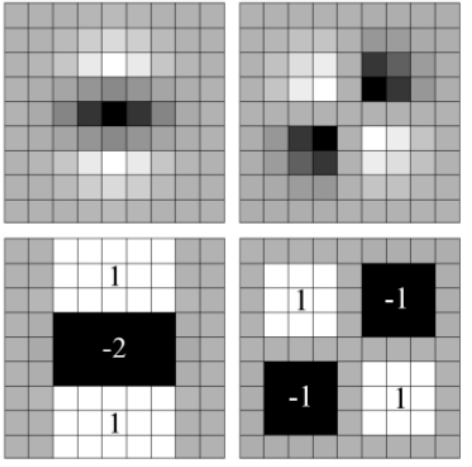
\includegraphics[width=0.55\textwidth]{img/surf4.PNG}
\caption{${L_{yy}(x,\sigma)}$ and${L_{xy}(x,\sigma)}$ Discretized
Gaussians and the approximations $D_{yy}$ and $D_{xy}$}
\label{fig:surf1}
\end{figure}

These approximate second order Gaussian derivatives and can be evaluated at a very low computational cost using integral images, and this is part of the reason why SURF is fast.

Now we can represent the determinant of the Hessian (approximated) as:

\begin{figure}[H]
\centering
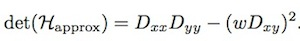
\includegraphics[width= 0.4\textwidth]{img/det.jpeg}

\label{fig:surfdet}
\end{figure}
and we can use 0.9 for w by Bay’s suggestion.

\subsection{ABOUT PYRAMID :}

In Sift, we use DOG to build image pyramids, the pyramid have several octaves, and there are several images layers in each octave. The difference between Sift pyramid and Surf pyramid is, in Sift, we use different scales of image; and in Surf, we use different scales of Gaussian masks, while the scale of image is always unaltered. By this, we save a lot of time by not downsampling image.

\begin{figure}[H]
\centering
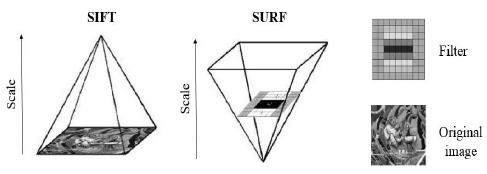
\includegraphics[width=0.6\textwidth]{img/surf2.png}
\caption{Where SIFT(left) downscales the image,
SURF(right) uses larger and larger filters}
\label{fig:surf2}
\end{figure}

 Instead of iteratively reducing the image size (left), the use of integral images allows the upscaling of the filter at constant cost (right).\\
 
 \subsection{ABOUT FEATURE DESCRIPTOR}
 In Sift, we use an orientation histogram, and find the largest orientation value and also those values that are over 80\% of the largest, and use these orientations as the main orientation of the feature descriptor. In Surf, we use the sum of the Haar wavelet response around the point of interest.

\begin{figure}[H]
\centering
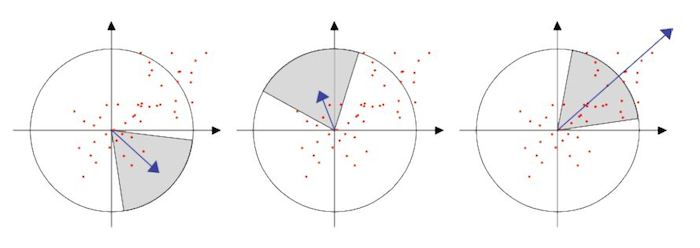
\includegraphics[width=0.6\textwidth]{img/surf3.jpg}
\caption{descriptor computation }
\label{fig:surf3}
\end{figure}

We first calculate the Haar wavelet responses in x and y direction within a circular neighborhood of radius 6s around the interest point, with s the scale at which the interest point was detected. We calculate the sum of vertical and horizontal wavelet responses in a scanning aria, then change the scanning orientation (add $\pi$/3), and recalculate, until we find the orientation with largest sum value, this orientation is the main orientation of feature descriptor.

Now it’s time to extract the descriptor. First we construct a square region centered around the feature point, and oriented along the main orientation we already got above, the size of this window is 20s,s is the scale at which the interest point was detected. Second we split this region up regularly into smaller 4$\times$4 square subregions, for each subregion, we compute Haar wavelet responses at 5$\times$5 regularly spaced sample points.


\begin{figure}[H]
\centering
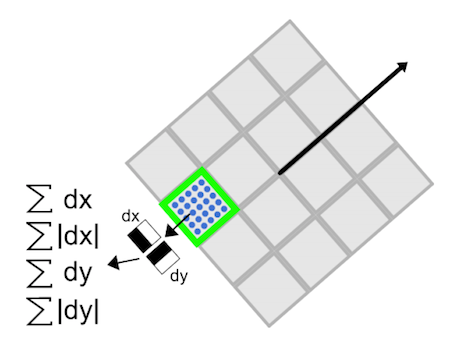
\includegraphics[width=0.5\textwidth]{img/surf5.png}
\caption{computation of dx and dy of Haar  }
\label{fig:surf5}
\end{figure}

We extract the sum of values of the responses in both x and y orientation, furthermore, we extract the sum of the absolute values of the responses, hence, each subregion has a 4-D descriptor vector v. Concatenating this for all 4$\times$4 subregions, our final descriptor is a 64-D vector. (In Sift, our descriptor is 128-D vector, so this is part of the reason that SURF is faster than Sift.)\\


\section{Differences and Preference :}
The two main advantages of SURF over SIFT is that SURF uses Laplacian of Gaussian so as to have a distinction
between background and foreground features, and secondly, SURF uses only 64 dimensional vector compared to 128 dimensional vector for SIFT . This helps in fast feature computation and also the quick matching capability.
The two different steps used by SURF to determine the local descriptor vectors are A. Keypoint Detection B. Keypoint Descriptor, which were  explained above \ref{} and \ref{}.

This makes Surf as our best candidate for gesture recognition  since it offers high number of stable features against Scale invariance and rotation invariance , of course lesser than Sift but it does not worth the Computational operations of up scaling pyramid used in sift Nor the \textbf{valuable }time consumed .

later on we will Experimentally demonstrate that Surf achieved  better accuracy than sift in Hand gesture Recognition  . However Even if Surf is less expensive than sift but still computationally expensive which is bad for our purposes ,Since what describe a Good HGR is its ability to interpret  and interact with the Signer performer in real time , That's where Fouriere descriptor Appears to give accurate and a Very Fast feature extractor which will meet our requirement for a robust and Real time application  .


\section{Fourier Shape Descriptor } \label{FDT}
The Fourier transformed coefficients from the Fourier
Descriptors of the shape represent the shape of the object in
the frequency domain. The general features of the shape can
be found in the lower frequency descriptors, while the higher
frequency descriptors contain information about the shape
details \cite{20}
Before applying Fourier transform on the shape boundary, it
is first normalized for matching purposes; this is done by
sampling the boundary of each shape to have the same number
of data points. The larger the number of sampled points the
more details in the representation of the shape this results in
more accurate matching. While a smaller number of sampled
points reduce the accuracy of the matching results but on the
other hand it will improve the computational efficiency. \\

After normalization we to apply Fourier transform to the
shape signature. A shape signature is any 1-D function
representing 2-D areas or boundaries. The shape signature we
used is complex coordinates. A complex coordinates function
is the complex form of the boundary coordinates \cite{20}. \\
\begin{gather}
    z_{i} = x_{i}+j y_{i} , i\in [1,N]
\end{gather}\\
For each shape we select N points with equal point
sampling. In order to facilitate the use of Fast Fourier
Transform (FFT), the number of sampled points is chosen to
be power of two. Assuming the number of sampled points is
N the Fourier transform gives N Fourier coefficients Cl. The
coefficients are usually called Fourier descriptors of the shape. 
\begin{gather}
C_{l}= \sum_{i=0}^{N-1} z_{i}e{\frac{-j 2\pi il}{N}} , l = 0,...,N-1
\end{gather}
The magnitude of the Fourier
Transform of this set forms a unique shape signature, which can be used for generalized
gesture classification.
In addition, this descriptor is rotationally invariant. Shifts in the silhouette contour
points, which is the cause of rotation, will be appear as phase delays in frequency
domain. However, since only the magnitude of the Fourier coefficients is considered,
the phase (or equivalently, the rotation) is ignored. So, this method is rotationally
invariant while remaining computationally fast\\


\textbf{Generating the Fourier Descriptor: }
\begin{enumerate}
    \item $X_{c} = \frac{1}{N}\sum_{n=0}^{N-1} x(i) , Y_{c} = \frac{1}{N}\sum_{n=0}^{N-1} y(i)  = 1$ , where N is number of hand object pixels 
    \item Take the magnitude of the N point DFT of these points :\\
              \textbf{ abs(FT{r[n]}) = a[m] , for m = 0..N-1 }.
    \item Normalize the Fourier coefficients by the DC value (Scale Invariance) .
    \item Keep the first 7 normalized coefficients (skip DC, which is always 1) .

\end{enumerate}


This is the Fourier Descriptor for a single shape.\\

\textbf{Make a Dictionary : } For a set of images of the same gesture, compute the average Fourier shape descriptor and add it to the dictionary with the same label.  Repeat for all desired gestures.

\textbf{Classification  : }Compute the Fourier descriptor for each new sample.  Compare it with each stored gesture in the dictionary using  Euclidean distance measure.  The label of the minimum distance is the desired gesture( Nearest Neighbor happens to be the most efficient method of classification )

\subsection{Covariance Matrix Approach :}
This approach \cite{21}
performs human action recognition by looking at a sequence of whole body silhouettes
over time, a silhouette tunnel, captured by the Kinect. A 13 dimensional feature vector
is defined, where 3 values are row, column, and time, 8 values are based on the shape of
the silhouette, and the last 2 are a measure of the temporal similarity.
However, this feature vector is general enough to work with hand silhouettes in addition
to full bodies. So, it is possible to modify the shape feature vector to work with static
hand gestures by reducing the dimensionality. This can be accomplished by removing
the time dependence and temporal similarity terms. The result is a generalized 10
dimensional feature vector applicable to static shape recognition.\\

\textbf{Create the Feature Vector :}\\
\begin{enumerate}
    \item Compute the 10-dimensional feature vector adapted from Guo \cite{21} : 
    
    \item f(x,y) = [x,y,de,dw,dn,ds,dne,dse,dnw]
    \begin{itemize}
        \item x = col , y=row
        \item d =  Euclidean distance from (x,y) to the nearest boundary point in the specified
direction \\
east, west, north, south, northeast, southwest, southeast, northwest
    \end{itemize}
    \item Scale Invariance 
    \begin{itemize}
        \item Divide each spatial feature by the square root of the silhouette area
     
    \end{itemize}
    \item Compute the Covariance Matrix: 
    \begin{itemize}
        \item $cov(f(\textbf{S}))=\frac{1}{|S|}\sum_{(x,y) \in S }(f(x,y)-\mu_{F})(f(x,y)-\mu_{F})^{T}$
        \item \textbf{S} = area of silhouettte 
        \item $\mu_{F} = \frac{1}{|S|}\sum_{(x,y) \in S } f(x,y) $
    \end{itemize}
    
\end{enumerate}
\textbf{Build a Dictionary }\\
For a set of images of the same gesture, compute the Covariance Matrix and add it to
the dictionary with the same label. Repeat for all desired gestures.\\
\textbf{Classification }\\
As noted in Guo \cite{21}, the set of all covariance matrices lie on a Riemannian
manifold. So, a Euclidean distance measure cannot be used. Instead, the distance
between two covariance matrices on this manifold is defined as:\\
$$d(C,C') = \sqrt{\sum_{k=1}^{10} (\ln \lambda_{k}(C,C'))^{2}}$$ \\
\texttt{where $\lambda_{k}(C,C')$ are generalized eigenvalues of C and C'\\
C = convariance Matrix of new sample ,  C' = Reference from dictionary  } \\

The label of the minimum distance gesture is used for classification .

\begin{table}[!h]
\centering
\caption{Pros and Con of Covariance approach }
\label{my-label}
\begin{tabular}{lllll}
\cline{1-2}
\multicolumn{1}{|l|}{\textbf{\begin{tabular}[c]{@{}l@{}}Pros:\\  1. Complex Gesture .\\  2. High accuracy.\\  3. Scale invariant.\end{tabular}}} & \multicolumn{1}{l|}{\textbf{\begin{tabular}[c]{@{}l@{}}Con :\\ 1. Not rotation Invariant . \\           \\        \\ \end{tabular}}} &  &  &  \\ \cline{1-2}
                                                                                                                                                 &                                                                                                           &  &  &  \\
                                                                                                                                                 &                                                                                                           &  &  &  \\
                                                                                                                                                 &                                                                                                           &  &  & 
\end{tabular}
\end{table}

\newpage
 
 \section{ Conclusion : }
 in this chapter we went through Two types of descriptors :\\
\textbf{the first} are  Local descriptors SIFT and SURF  descriptors that typically involves more intense computations and algorithms, often requiring floating point
calculations, and may consume considerable memory.but generally they give a high  accuracy Additionally to their stable performance even against scale variation and Rotation variation too , the following table is summarizing the Differences of these two descriptors :

\begin{table}[!h]
\centering
\caption{COMPARISON OF SIFT AND SURF}
\label{surfvssift}
\begin{tabular}{l|l|l|ll}
\cline{2-3}
\textbf{}                                                                                     & \textbf{SIFT}                                                                                                                                                     & \textbf{SURF}                                                                                                                             &  &  \\ \cline{1-3}
\multicolumn{1}{|l|}{\textbf{\begin{tabular}[c]{@{}l@{}}Keypoint\\ Detection\end{tabular}}}   & \textbf{\begin{tabular}[c]{@{}l@{}}Different scale image\\ convoluted with\\ Gaussian function\end{tabular}}                                                      & \textbf{\begin{tabular}[c]{@{}l@{}}Original Image is\\ convoluted with\\ Different scale box\\ filter\end{tabular}}                       &  &  \\ \cline{1-3}
\multicolumn{1}{|l|}{\textbf{\begin{tabular}[c]{@{}l@{}}Keypoint\\ Description\end{tabular}}} & \textbf{\begin{tabular}[c]{@{}l@{}}Gradient amplitude of\\ a square area is\\ calculated with\\ maximum gradient\\ strength as the main\\ direction\end{tabular}} & \textbf{\begin{tabular}[c]{@{}l@{}}A Haar Wavelet response\\  is used to\\ calculate \\ each sector in\\ a \\ circular area\end{tabular}} &  &  \\ \cline{1-3}
\multicolumn{1}{|l|}{\textbf{Dimensions}}                                                     & 128                                                                                                                                                               & 64                                                                                                                                        &  &  \\ \cline{1-3}
\end{tabular}
\end{table}



\textbf{The second } are Basis Space descriptors   , A basis space is composed of a set of functions, the basis functions, which are
composed together as a set, such as a series like the Fourier series and covariance Matrix  . \\
Fourier descriptors represent feature data as sine and cosine terms, which can be
observed in a Fourier Power Spectrum. The Fourier series, Fourier transform, and Fast
Fourier transform are used for a wide range of signal analysis, including 1D, 2D, and 3D
problems. No discussion of image processing or computer vision is complete without
Fourier methods .

With this summary we are done from Feature detection / extraction and we will move on to the next Phase of building  our HGR System , which is  Feature classification using Machine learning algorithms that's going to be the goal of next section .

\chapter{Machine Learning}

\section{What Is Machine Learning?}

Machine learning is a sub-field of artificial intelligence (AI) concerned with algorithms
that allow computers to learn. What this means, in most cases, is that an
algorithm is given a set of data and infers information about the properties of the
data and that information allows it to make predictions about other data that it
might see in the future. This is possible because almost all nonrandom data contains
patterns, and these patterns allow the machine to generalize, in order to do as such, it
trains a model with what it determines are the important aspects of the data.\\
\newline
To understand how models come to be, consider a simple example in the otherwise
complex field of email filtering. Suppose you receive a lot of spam that contains the
words “online pharmacy.” As a human being, you are well equipped to recognize patterns,
and you quickly determine that any message with the words “online pharmacy” is spam and should be moved directly to the trash, this is a generalization you have,
in fact, created a mental model of what is spam.\\ After you report several of these
messages as spam, a machine-learning algorithm designed to filter spam should be
able to make the same generalization.\\
\newline
There are many different machine-learning algorithms, all with different strengths
and suited to different types of problems. Some, such as decision trees, are transparent,
so that an observer can totally understand the reasoning process undertaken by
the machine. Others, such as neural networks, are blackbox, meaning that they produce
an answer, but it’s often very difficult to reproduce the reasoning behind it.
Many machine-learning algorithms rely heavily on mathematics and statistics, according to the definition we gave earlier, we could even say that simple correlation
analysis and regression are both basic forms of machine learning. 
\section{Supervised Machine Learning}

The majority of practical machine learning uses supervised learning.\\
Supervised learning is where we have input variables (x) and an output variable (Y) and we use an algorithm to learn the mapping function from the input to the output.
\newline
$Y = f(X)$
\newline
The goal is to approximate the mapping function so well that when we have new input data (x) that we can predict the output variables (Y) for that data.
\newline
It is called supervised learning because the process of an algorithm learning from the training dataset can be thought of as a teacher supervising the learning process.\\ We know the correct answers, the algorithm iteratively makes predictions on the training data and is corrected by the teacher. Learning stops when the algorithm achieves an acceptable level of performance.\\
\newline
Supervised learning problems can be further grouped into regression and classification problems.\\
\newline
\textbf{Classification:} A classification problem is when the output variable is a category, such as “red” or “blue” or “disease” and “no disease”.\\ \textbf{Regression:}  A regression problem is when the output variable is a real value, such as “dollars” or “weight”.
Some common types of problems built on top of classification and regression include recommendation and time series prediction respectively.

Some popular examples of supervised machine learning algorithms are:\\

Linear regression for regression problems.\\

Random forest for classification and regression problems.\\

Support vector machines for classification problems.



\section{Unsupervised learning}

In supervised learning, the aim is to learn a mapping from the input to
an output whose correct values are provided by a supervisor.\\
In unsupervised
learning, there is no such supervisor and we only have input data.
The aim is to find the regularities in the input, there is a structure to the
input space such that certain patterns occur more often than others, and we want to see what generally happens and what does not. In statistics, this is called density estimation.
One method for density estimation is clustering where the aim is to
find clusters or groupings of input.\\ 
Some popular examples of unsupervised learning algorithms are:


\begin{itemize}
  \item k-means for clustering problems.
  \item Apriori algorithm for association rule learning problems.
\end{itemize}

\par



\section{Support Vector Machines (SVM) }\label{sec:svm}

Support Vector Machines are based on the concept of decision planes that define decision boundaries. A decision plane is one that separates between a set of objects having different class memberships. A schematic example is shown in the illustration below. In this example, the objects belong either to class GREEN or RED. The separating line defines a boundary on the right side of which all objects are GREEN and to the left of which all objects are RED. Any new object (white circle) falling to the right is labeled, i.e., classified, as GREEN (or classified as RED should it fall to the left of the separating line).


\begin{figure}[H]
\centering
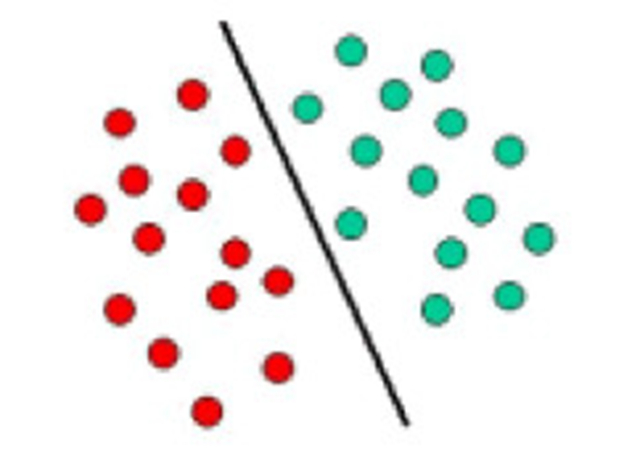
\includegraphics[width=0.3\textwidth]{img/svm1.png}
\caption{example of linear Hyperplan seperating Green data from Red data }
\label{122 }
\end{figure}


The above is a classic example of a linear classifier, i.e., a classifier that separates a set of objects into their respective groups (GREEN and RED in this case) with a line. Most classification tasks, however, are not that simple, and often more complex structures are needed in order to make an optimal separation, i.e., correctly classify new objects (test cases) on the basis of the examples that are available (train cases). This situation is depicted in the illustration below. Compared to the previous schematic, it is clear that a full separation of the GREEN and RED objects would require a curve (which is more complex than a line). Classification tasks based on drawing separating lines to distinguish between objects of different class memberships are known as hyperplane classifiers. Support Vector Machines are particularly suited to handle such tasks


\begin{figure}[H]
\centering
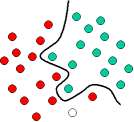
\includegraphics[width=0.3\textwidth]{img/svm2.png}
\caption{Non linear Example of data  }
\label{123 }
\end{figure}

The illustration below shows the basic idea behind Support Vector Machines. Here we see the original objects (left side of the schematic) mapped, i.e., rearranged, using a set of mathematical functions, known as kernels. The process of rearranging the objects is known as mapping (transformation). Note that in this new setting, the mapped objects (right side of the schematic) is linearly separable and, thus, instead of constructing the complex curve (left schematic), all we have to do is to find an optimal line that can separate the GREEN and the RED objects.

\begin{figure}[H]
\centering
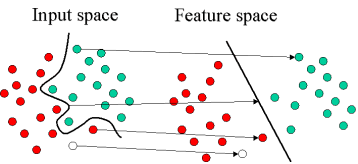
\includegraphics[width=0.5\textwidth]{img/SVMIntro3.png}
\caption{Non linear separated using kernel (higher dimension) }
\label{124 }
\end{figure}


\subsection{Hard-Margin SVM}
The SVM technique is a classifier that finds a hyperplane or a function $g(x) = {\omega}^T +  b$   that correctly separates two classes with a maximum margin.figure below shows a separating hyperplane corresponding to a hard-margin SVM (also called a linear SVM).

\begin{figure}[H]
\centering
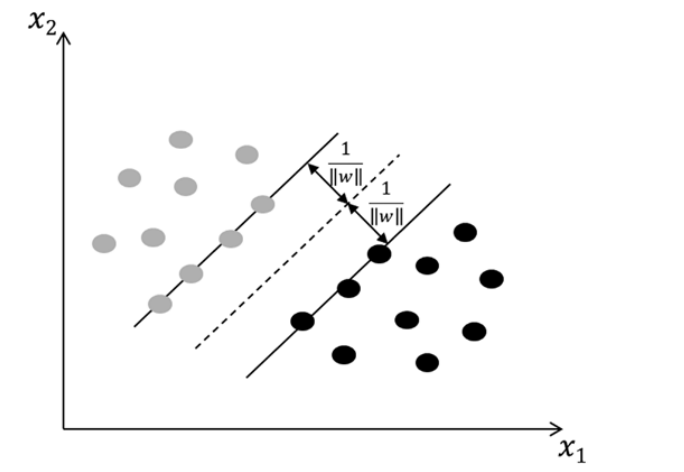
\includegraphics[width=0.5\textwidth]{img/hardmargin.PNG}
\caption{ Hard-maximum-margin separating hyperplane. }
\label{125 }
\end{figure}


\subsection{Soft-Margin SVM}

When the data are not completely separable, as with the points marked by a X in Figure below  , slack variables Xi  are introduced to the SVM objective function to allow error in the misclassification. SVM, in this case, is not searching for the hard margin, which will classify all data flawlessly. Instead, SVM is now a soft-margin classifier; that is, SVM is classifying most of the data correctly, while allowing the model to misclassify a few points in the vicinity of the separating boundary

\begin{figure}[H]
\centering
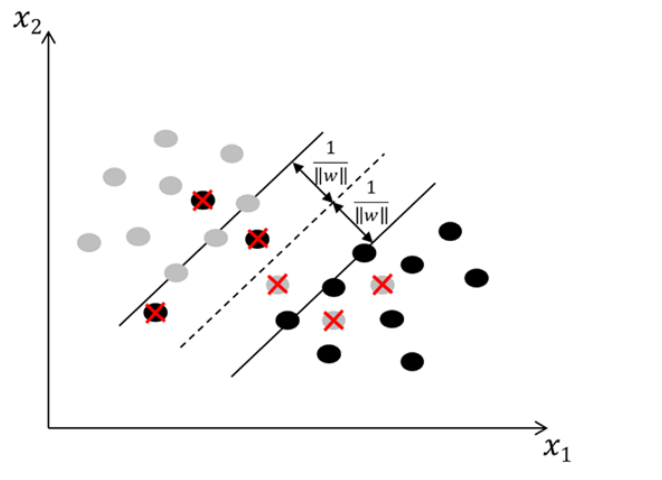
\includegraphics[width=0.5\textwidth]{img/softmargin.PNG}
\caption{  A few misclassifications, as part of soft-margin SVM . }
\label{126 }
\end{figure}


\subsection{Kernels}

When a problem is not linearly separable in input space, soft-margin SVM cannot find a robust separating
hyperplane that minimizes the number of misclassified data points and that generalizes well. For that, a kernel can be used to transform the data to a higher-dimensional space, referred to as kernel space, where data will be linearly separable. In the kernel space a linear hyperplane can thus be obtained to separate the different classes involved in the classification task instead of solving a high-order separating hypersurface in the input space. This is an attractive method, because the overhead on going to kernel space is insignificant compared with learning a nonlinear surface. A kernel should be a Hermitian and positive semidefinite matrix and needs to satisfy Mercer’s theorem, which translates into evaluating the kernel or Gram matrix on all pairs of data points as positive and semidefinite, forming
\newline 
\newline
$K(\small{x,u})=\sum\limits_{r} \phi(x)\phi(u) $ .

where $\phi(x) $ belongs to the Hilbert space.
\newline
$$\int \int K(x,u) g(x) g(u) du dx \geq 0 \ \ \ \ \forall g(x) , \ where \int g^2(x) dx < +\infty$$
\\
\newline 
Some popular kernel functions include
\newline
\newline


\begin{itemize}

  \item  Linear kernel  : 
  \begin{align*}
  \mathlarger {K(x,u)=  x^{T}.u  }
   \end{align*}
  \item Polynomial function: 
  \begin{align*}
  K(x,u)=(ax^{T}u + c)^{q} ,\, q>0.
  \end{align*}
  \item Gaussian radial basis function (RBF): 
\begin{align*} 
 K(x,u) = e^{\mathlarger{\frac{\mathbf{-\| x -  u\|^2}}{\mathbf{\sigma^2} } }}
\end{align*}
   
  \item  Hyperbolic tangent (sigmoid):
    \begin{equation}
      K(\mathbf x, \mathbf u) = \tanh(\mathbf {\beta} \mathbf x^{T} \mathbf u - \mathbf{\delta})^p
    \end{equation}
    
    \item Laplacian radial basis function : 
    
    \begin{align*} 
      K(x,u) = e^{\mathlarger{\frac{-\| x -  u\|}{\sigma} } }
     \end{align*}
    
\end{itemize}

Kernel selection is heavily dependent on the data specifics. For instance, the linear kernel—the simplest
of all—is useful in large sparse data vectors. However, it ranks behind the polynomial kernel, which avoids
zeroing the Hessian. \\The polynomial kernel is widely used in image processing, The Gaussian and Laplace RBFs are general-purpose kernels
that are mostly applied in the absence of prior knowledge. \\A kernel matrix that ends up being diagonal indicates that the feature space is redundant and that another kernel should be tried after feature reduction.\\
\newline
\newline
\textbf{
Note} that when kernels are used to transform the feature vectors from input space to kernel space for linearly non-separable datasets, the kernel matrix computation requires massive memory and computational
resources, for big data . 

\par
\par

\section{Nearest Neighbour Based Classifiers}
One of the simplest decision procedures that can be used for classification is the
nearest neighbour (NN) rule. It classifies a sample based on the category of its nearest
neighbour.When large samples are involved,it can be shown that this rule has a
probability of error which is less than twice the optimum error
—hence there is less
than twice the probability of error compared to any other decision rule. The nearest
neighbour based classifiers use some or all the patterns available in the training set
to classify a test pattern. These classifiers essentially involve finding the similarity
between the test pattern and every pattern in the training set.

\subsection{Nearest Neighbour Algorithm}
The nearest neighbour algorithm assigns to a test pattern the class label of its closest
neighbour

% Insert the algorith

\begin{algorithm}[H]
\SetAlgoLined

 initialization\;
 $ A=(X_{1},\omega_{1}),(X_{2},\omega_{2}),....,(X_{n},\omega_{n}) \ // A\ is\ the\ set\ of\ N\ training\ pattern $\\
 
 
$ //where\  X_{i}\ is\ of\ dimension\ n\ and\  \omega_{i}\ is\ the\ class\ label\ of\ the\ i^{th}\ pattern $\\
 
 
 $d(u,x) = \sqrt{\sum_{k=0}^{N} (u_{i}-x_{i})^{2}}  // \ Euclidean\ distance\ measure $\\ 

 \While{ i \neq N }{ // N samples
 
  d(X_{t},X_{i}) = min {D(X_{t},X_{i})}\; 
 
 }
 
 $ X_{t} = \omega_{k} $ \\
 
 $ pattern\ X_{t}\ is\ assigned\ to\ a\ class\ \omega_{k}\ associated\ with\  X_{k} $
 
 \caption{Algorithm for NN}
\end{algorithm}

\vspace{5mm}
\textbf{Example of the algorithm} :\newline 
$ X1 = (0.8, 0.8, 1), X2 = (1.0, 1.0, 1), X3 = (1.2, 0.8, 1)$\\
$X4 = (0.8, 1.2, 1), X5 = (1.2, 1.2, 1), X6 = (4.0, 3.0, 2)$\\
$X7 = (3.8, 2.8, 2), X8 = (4.2, 2.8, 2), X9 = (3.8, 3.2, 2)$\\
$X10 = (4.2, 3.2, 2), X11 = (4.4, 2.8, 2), X12 = (4.4, 3.2, 2)$\\
$X13 = (3.2, 0.4, 3), X14 = (3.2, 0.7, 3), X15 = (3.8, 0.5, 3)$\\
$X16 = (3.5, 1.0, 3), X17 = (4.0, 1.0, 3), X18 = (4.0, 0.7, 3)$

\begin{figure}[H]
\centering
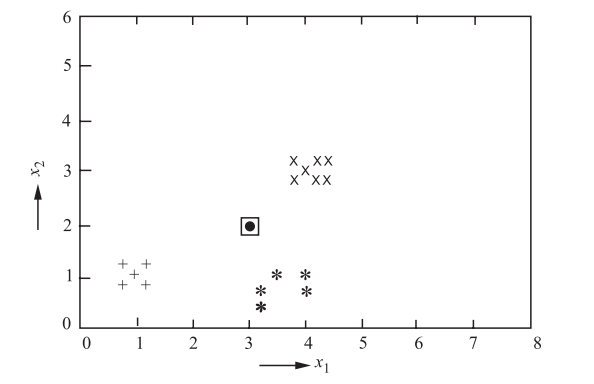
\includegraphics[width=0.6\textwidth]{img/nn-example.PNG}
\caption{ Example data set }
\label{fig:NN}
\end{figure}

For each pattern, the first two numbers in the triplets gives the first and second
features, and the third number gives the class label of the pattern.
This can be seen plotted in Figure \ref{fig:NN}. Here ‘‘+’’ corresponds to Class 1, ‘‘X’’
corresponds to Class 2 and ‘‘*’’ corresponds to Class 3.
Now if there is a test pattern P = (3.0, 2.0), it is necessary to find the distance
from P to all the training patterns.
Let the distance between X and P be the Euclidean distance

$$D(X,P) = \sqrt{(X1 - P1)^{2} + (X2 - P2 )^{2} }$$
\newline
The distance from a point P to every point in the set can be computed using the above formula. For P = (3.0, 2.0), the distance to X1 is :
$D(X1,P) = \sqrt{(0.8 - 3.0)^{2} + (0.8 - 2.0 )^{2} } = 2.51 $ \\
We find, after calculating the distance from all the training points to P, that the closest
neighbour of P is X16, which has a distance of 1.12 from P and belongs to Class 3.
Hence P is classified as belonging to Class 3.
\subsection{Variants of the NN Algorithm}
\subsubsection{k-Nearest Neighbour (kNN) Algorithm}
In pattern recognition, the k-nearest neighbors algorithm (k-NN) is a non-parametric method used for classification and regression.  In both cases, the input consists of the k closest training examples in the feature space. The output depends on whether k-NN is used for classification or regression:
\begin{itemize}
\item In k-NN classification, the output is a class membership. An object is classified by a majority vote of its neighbors, with the object being assigned to the class most common among its k nearest neighbors (k is a positive integer, typically small). 
\item In k-NN regression, the output is the property value for the object. This value is the average of the values of its k nearest neighbors.
\end{itemize}

k-NN is a type of instance-based learning, or lazy learning, where the function is only approximated locally and all computation is deferred until classification. The k-NN algorithm is among the simplest of all machine learning algorithms.\\ Both for classification and regression, it can be useful to assign weight to the contributions of the neighbors, so that the nearer neighbors contribute more to the average than the more distant ones. For example, a common weighting scheme consists in giving each neighbor a weight of 1/d, where d is the distance to the neighbor.\\ The neighbors are taken from a set of objects for which the class (for k-NN classification) or the object property value (for k-NN regression) is known. This can be thought of as the training set for the algorithm, though no explicit training step is required.

\subsubsection{Modified k-Nearest Neighbour (MkNN) Algorithm}
This algorithm is similar to the kNN algorithm, inasmuch as it takes the k nearest
neighbours into consideration. The only difference is that these k nearest neighbours
are weighted according to their distance from the test point. It is also called
the distance-weighted k-nearest neighbour algorithm. Each of the neighbours is
associated with the weight w which is defined as
$$ \left\{\begin{matrix}
\frac{ \mathlarger{d_{k} - d_{j}}} { \mathlarger{{d_{k} - d_{1}} }} \   \ if \ d_{k} \neq d_{1} \\ 
\mathlarger{1} \  \   \     \ if \ d_{k}  =  d_{1}
\end{matrix}\right.   $$

where j = 1, .., k. The value of wj varies from a maximum of 1 for the nearest
neighbour down to a minimum of zero for the most distant. Having computed the
weights wj, the MkNN algorithm assigns the test pattern P to that class for which the
weights of the representatives among the k nearest neighbours sums to the greatest
value.\\
Instead of using the simple majority rule, it can be observed that MkNN employs
a weighted majority rule. This would mean that outlier patterns have lesser effect on
classification

%%%%%%%%%%%%%%%%%%%%%%%%%
\section{Artificiel Neural Network}
The architecture of an artificial neural network defines how its several neurons are
arranged, or placed, in relation to each other. These arrangements are structured
essentially by directing the synaptic connections of the neurons.
The topology of a given neural network, within a particular architecture, can be
defined as the different structural compositions it can assume. In other words, it is
possible to have two topologies belonging to the same architecture, where the first
topology is composed of 10 neurons, and the second is composed of 20 neurons.
Moreover, one can consist of neurons with logistic activation function, while the
other one can consist of neurons with the hyperbolic tangent as the activation
function.
On the other hand, training a particular architecture involves applying a set of
ordinated steps to adjust the weights and thresholds of its neurons. Hence, such
adjustment process, also known as learning algorithm, aims to tune the network so
that its outputs are close to the desired values


\subsection{Main Architectures of Artificial Neural Networks}

In general, an artificial neural network can be divided into three parts, named layers,which are known as:\\

\textbf{(a) Input layer}
This layer is responsible for receiving information (data), signals, features, or measurements from the external environment. These inputs (samples or patterns) are usually normalized within the limit values produced by activation functions. This normalization results in better numerical precision for the mathematical operations performed by the network.\\

\textbf{(b) Hidden, intermediate, or invisible layers}
These layers are composed of neurons which are responsible for extracting patterns associated with the process or system being analyzed. These layers perform most of the internal processing from a network.\\

\textbf{(c) Output layer}
This layer is also composed of neurons, and thus is responsible for producing and presenting the final network outputs, which result from the processing performed by the neurons in the previous layers.
\\
\\
The main architectures of artificial neural networks, considering the neuron disposition, as well as how they are interconnected and how its layers are composed, can be divided as follows:\textbf{(3.6.2)} single-layer feedforward network,\textbf{(3.6.3)} multilayer feedforward networks, \textbf{(3.6.4)} recurrent networks and \textbf{(3.6.5)} mesh networks

\subsection{Single-Layer Feedforward Architecture}
This artificial neural network has just one input layer and a single neural layer,
which is also the output layer. \ref{fig:ann1} illustrates a simple-layer feedforward network composed of n inputs and m outputs.
The information always flows in a single direction (thus, unidirectional), which is from the input layer to the output layer. From \ref{fig:ann1}, it is possible to see that in networks belonging to this architecture, the number of network outputs will always
coincide with its amount of neurons. These networks are usually employed in pattern classification and linear filtering problems.
Among the main network types belonging to feedforward architecture are the Perceptron and the ADALINE, whose learning algorithms used in their training processes are based respectively on Hebb’s rule and Delta rule, as it will be discussed
in the next chapters.


\begin{figure}[H]
\centering
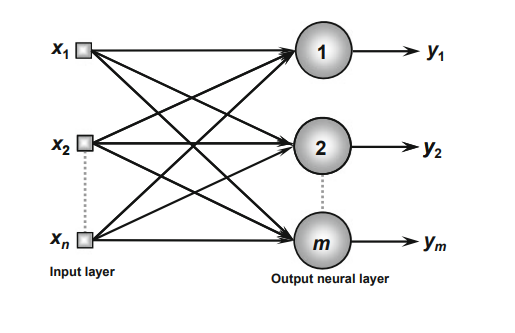
\includegraphics[width=0.5\textwidth]{img/ann1.PNG}
\caption{  Example of a single-layer feedforward network }
\label{fig:ann1}
\end{figure}

\subsection{Multiple-Layer Feedforward Architectures}
Differently from networks belonging to the previous architecture, feedforward
networks with multiple layers are composed of one or more hidden neural layers
(\ref{fig:ann2}). They are employed in the solution of diverse problems, like those related
to function approximation, pattern classification, system identification, process
control, optimization, robotics, and so on.
\ref{fig:ann2} shows a feedforward network with multiple layers composed of one
input layer with n sample signals, two hidden neural layers consisting of n1 and n2
neurons respectively, and, finally, one output neural layer composed of m neurons
representing the respective output values of the problem being analyzed.
Among the main networks using multiple-layer feedforward architectures are the
Multilayer Perceptron (MLP) and the Radial Basis Function (RBF), whose learning
algorithms used in their training processes are respectively based on the generalized
delta rule and the competitive/delta rule. These concepts will be addressed in the
next chapters.
From \ref{fig:ann2}, it is possible to understand that the amount of neurons composing
the first hidden layer is usually different from the number of signals composing the
input layer of the network. In fact, the number of hidden layers and their respective
amount of neurons depend on the nature and complexity of the problem being
mapped by the network, as well as the quantity and quality of the available data
about the problem. Nonetheless, likewise for simple-layer feedforward networks,
the amount of output signals will always coincide with the number of neurons from
that respective layer.

\begin{figure}[H]
\centering
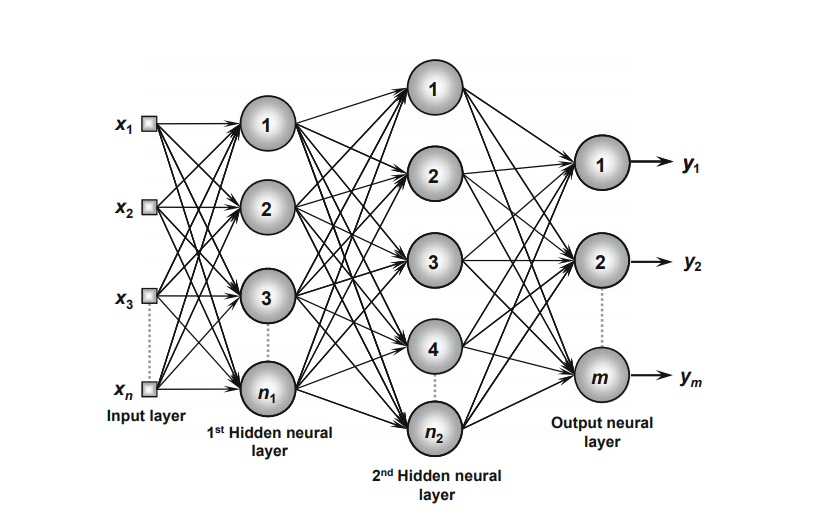
\includegraphics[width=0.7\textwidth]{img/ann2.PNG}
\caption{  Example of a feedforward network with multiple layers }
\label{fig:ann2}
\end{figure}


\subsection{Recurrent or Feedback Architecture}
In these networks, the outputs of the neurons are used as feedback inputs for other
neurons. The feedback feature qualifies these networks for dynamic information
processing, meaning that they can be employed on time-variant systems, such as
time series prediction, system identification and optimization, process control, and
so forth.
Among the main feedback networks are the Hopfield and the Perceptron with
feedback between neurons from distinct layers, whose learning algorithms used in
their training processes are respectively based on energy function minimization and
generalized delta rule, as will be investigated in the next chapters.
\ref{fig:ann3} illustrates an example of a Perceptron network with feedback, where
one of its output signals is fed back to the middle layer.
Thus, using the feedback process, the networks with this architecture produce
current outputs also taking into consideration the previous output values.
\begin{figure}[H]
\centering
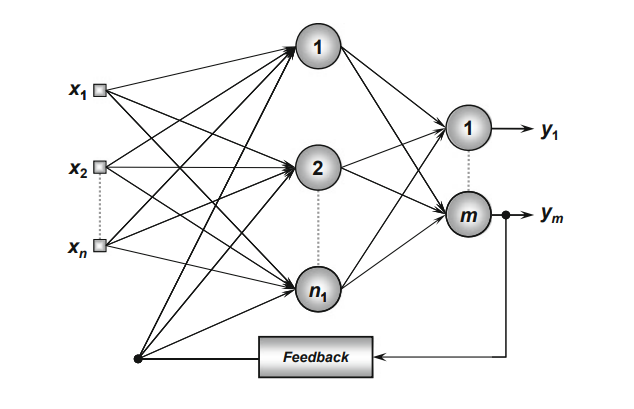
\includegraphics[width=0.65\textwidth]{ann3.PNG}
\caption{ Example of a recurrent network }
\label{fig:ann3}
\end{figure}

\subsection{Mesh Architectures}
The main features of networks with mesh structures reside in considering the spatial
arrangement of neurons for pattern extraction purposes, that is, the spatial localization
of the neurons is directly related to the process of adjusting their synaptic
weights and thresholds. These networks serve a wide range of applications and are
used in problems involving data clustering, pattern recognition, system optimization,
graphs, and so forth.
The Kohonen network is the main representative of mesh architectures, and its
training is performed through a competitive process, as will be described in the
following chapters. \ref{fig:ann4} illustrates an example of the Kohonen network
where its neurons are arranged within a two-dimensional space.
\begin{figure}[H]
\centering
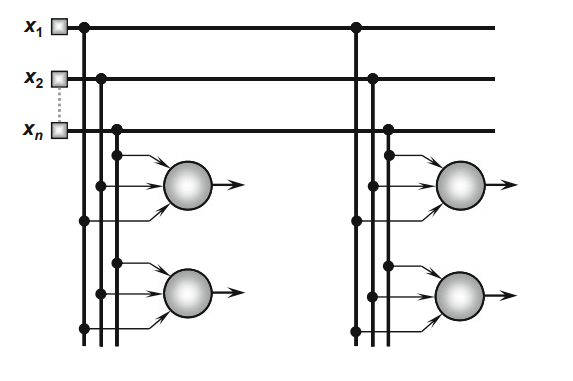
\includegraphics[width=0.5\textwidth]{img/ann4.PNG}
\caption{ Structure of a mesh network }
\label{fig:ann4}
\end{figure}


\subsection{Training Processes and Properties of Learning}
One of the most relevant features of artificial neural networks is their capability of
learning from the presentation of samples (patterns), which expresses the system
behavior. Hence, after the network has learned the relationship between inputs and
outputs, it can generalize solutions, meaning that the network can produce an output
which is close to the expected (or desired) output of any given input values.
Therefore, the training process of a neural network consists of applying the
required ordinated steps for tuning the synaptic weights and thresholds of its
neurons, in order to generalize the solutions produced by its outputs.
The set of ordinated steps used for training the network is called learning
algorithm. During its execution, the network will thus be able to extract discriminant
features about the system being mapped from samples acquired from the
system.
Usually, the complete set containing all available samples of the system behavior
is divided into two subsets, which are called training subset and test subset. The
training subset, composed of 60–90\% of random samples from the complete set,
will be used essentially in the learning process. On the other hand, the test subset,
which is composed of 10–40 \% from the complete sample set, will be used to verify
if the network capabilities of generalizing solutions are within acceptable levels,
thus allowing the validation of a given topology. Nonetheless, when dimensioning these subsets, statistical features of the data must also be considered.
During the training process of artificial neural networks, each complete presentation
of all the samples belonging to the training set, in order to adjust the
synaptic weights and thresholds, will be called training epoch.
\newline
\section{ K-Means Clustering }
K-means \cite{kmeans} is one of the simplest unsupervised learning algorithms that solve the well known clustering problem. \\ K-Means clustering intends to partition n objects into k clusters in which each object belongs to the cluster with the nearest mean. This method produces exactly k different clusters of greatest possible distinction. The best number of clusters k leading to the greatest separation (distance) is not known as a priori and must be computed from the data. The objective of K-Means clustering is to minimize total intra-cluster variance, or, the squared error function:
\begin{figure}[H]
\centering
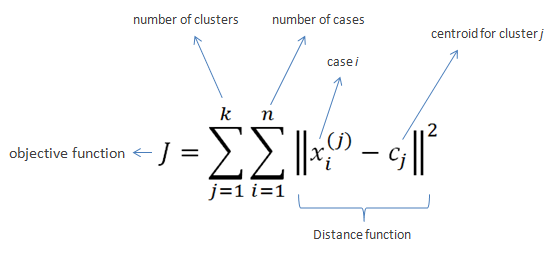
\includegraphics[width=0.5\textwidth]{img/ckmeans.png}
\end{figure}

 The algorithm as described by \cite{kmeans} starts with a random set of $k$ center-points ($\mu$). During each update step, all observations $x$ are assigned to their nearest center-point (see equation \ref{eqn:kmeans_assign_step}). In the standard algorithm, only one assignment to one center is possible. If multiple centers have the same distance to the observation, a random one would be chosen.

\begin{equation}
S_i^{(t)} = \big \{ x_p : \big \| x_p - \mu^{(t)}_i \big \|^2 \le \big \| x_p - \mu^{(t)}_j \big \|^2 \ \forall j, 1 \le j \le k \big\}
\label{eqn:kmeans_assign_step}
\end{equation}

Afterwards, the center-points are repositioned by calculating the mean of the assigned observations to the respective center-points (see \eqnref{kmeans_update_step}).

\begin{equation}
\mu^{(t+1)}_i = \frac{1}{|S^{(t)}_i|} \sum_{x_j \in S^{(t)}_i} x_j
\label{eqn:kmeans_update_step}
\end{equation}

The update process reoccurs until all observations remain at the assigned center-points and therefore the center-points would not be updated anymore.

% sample images

\begin{figure}
\centering
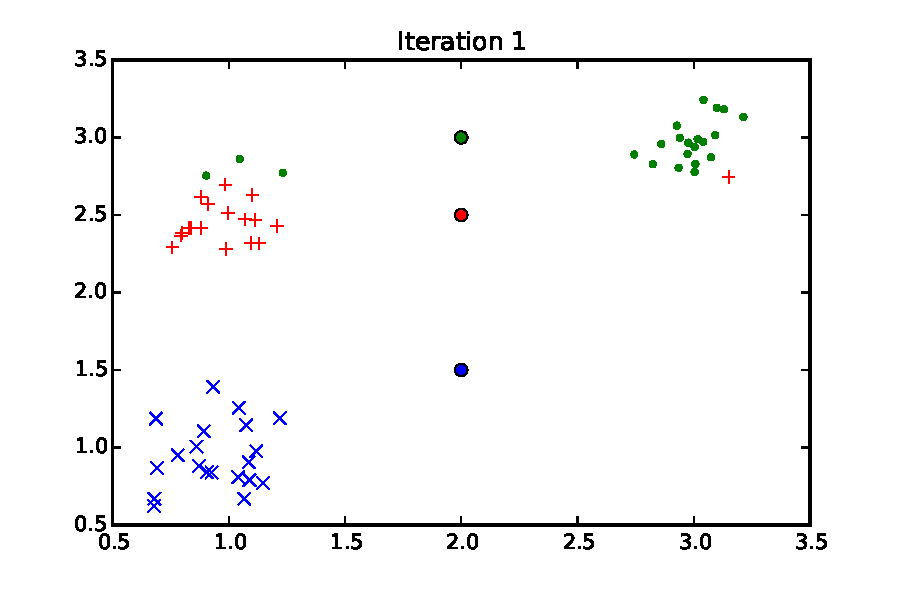
\includegraphics[width=0.6\linewidth]{img/iteration01}
\caption{k-Means: Possible initial centroid positions}
\label{fig:kmeans:iteration01}
\end{figure}

\begin{figure}
\centering
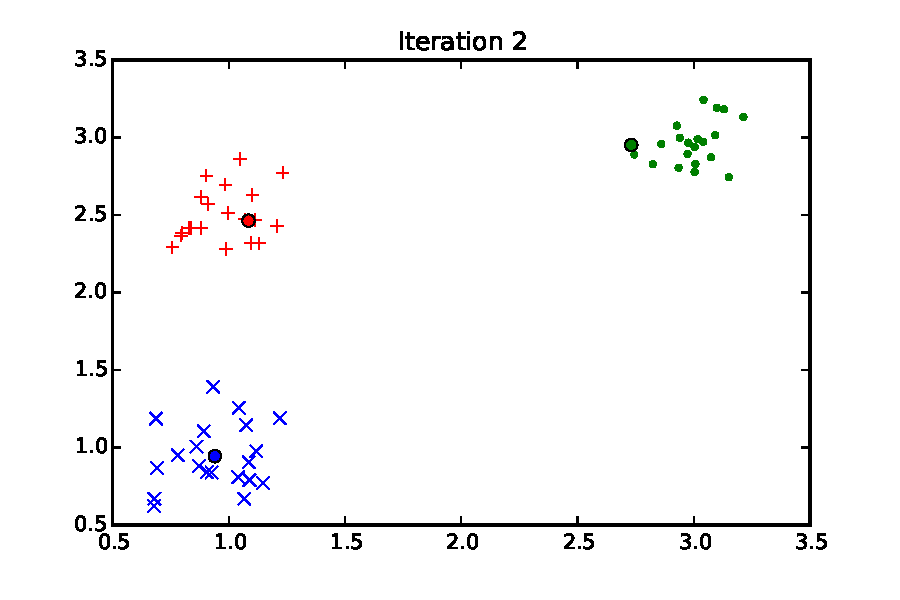
\includegraphics[width=0.6\linewidth]{img/iteration02}
\caption{k-Means: First iteration}
\label{fig:kmeans:iteration02}
\end{figure}

\begin{figure}
\centering
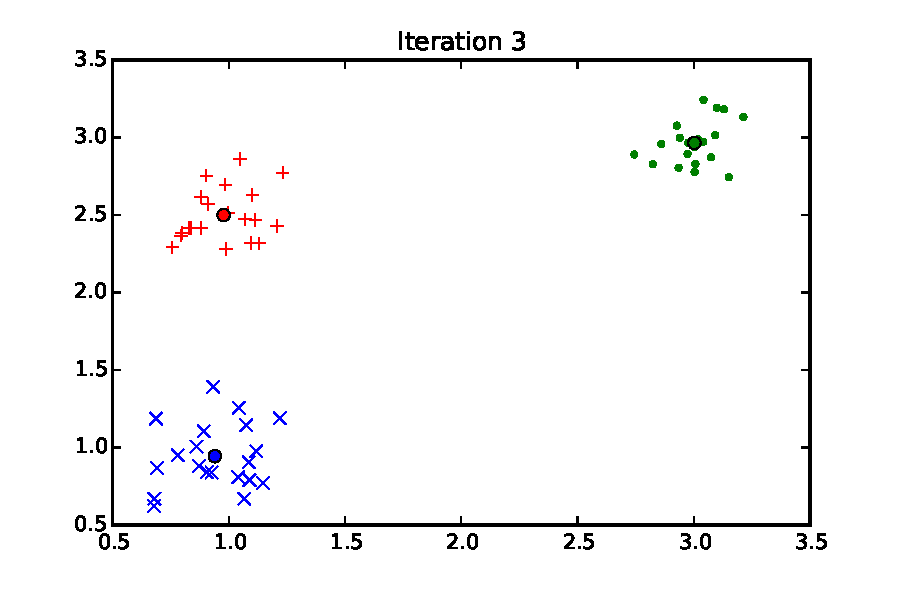
\includegraphics[width=0.6\linewidth]{img/iteration03}
\caption{k-Means: Second iteration}
\label{fig:kmeans:iteration03}
\end{figure}


This means that the k-means algorithm tries to optimize the objective function \ref{eqn:kmeans_objective_function}. As there is only a finite number of possible assignments for the amount of centroids and observations available and each iteration has to result in better solution, the algorithm always ends in a local minimum.

\begin{equation}
J = \sum_{n=1}^{N} \sum_{k=1}^{K} r_{nk} ||x_n - \mu_k||^2
\label{eqn:kmeans_objective_function}
\end{equation}

\[
\text{with } \\
r_{nk} = \begin{cases}
%1 & \text{if } k = \arg \min_j ||x_n - \mu_j||^2 \\
1 & x_n \in S_k \\
0 & \text{otherwise}
\end{cases}
\]

% minimize graph image

The main problem of k-means is its dependency on the initially chosen centroids. The centroids could end up in splitting common data points whilst other, separated points get grouped together if some of the centroids are more attracted by outliers. This points will get pulled to the same group of data points as shown in figure \ref{fig:kmeans_bad}.


\begin{figure}[h]
\centering
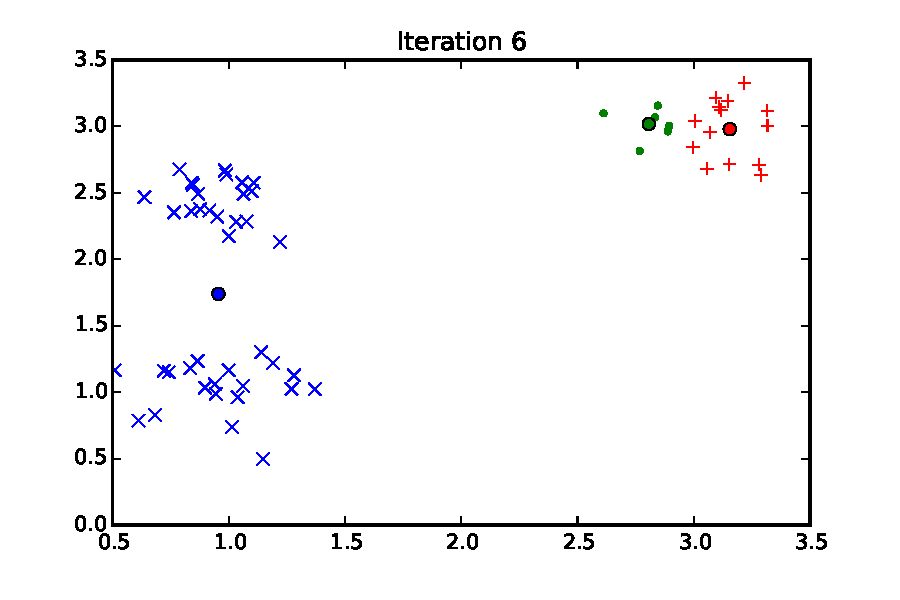
\includegraphics[width=0.6\linewidth]{img/kmeans_bad}
\caption{k-Means: Badly chosen initial center points}
\label{fig:kmeans_bad}
\end{figure}

The most common approach is to perform multiple clusterings with different start positions. Afterwards the clustering, which occurred most is considered as correct. Another, newer approach is the so called k-means++ by Arthur and Vassilvitskii \cite{Arthur}. This extension to the k-means algorithm tries to distribute the initial centroids over the given data to minimize the probability of bad outcomes. The initial points are set according to the authors by the following steps

\begin{enumerate}
    \item Take uniformly a random data point from the data $X$ and mark it as centroid $c_1$
    \item Choose another centroid $c_i$ with the probability $\frac{D(x)^2}{\sum_{x \in X} D(x)^2}$ where $D(x)$ denotes the shortest distance from the data point $x$ to its closest, already chosen centroid.
    \item Repeat 2. until all $k$ initial centroids are chosen.
\end{enumerate}

Afterwards, the standard k-means algorithm as described above is performed. The authors also showed that with this initialization algorithm, k-means++ approximately can be computed in $O(\log n)$, compared to $O(n^{dk+1} \log n)$ for the standard algorithm.


\newpage
\section{Model Selection } \label{ms}
Model selection is the process of choosing between different machine learning approaches - e.g. SVM, logistic regression, etc - or choosing between different hyperparameters or sets of features for the same machine learning approach - e.g. deciding between the polynomial degrees/complexities for linear regression.\\
The choice of the actual machine learning algorithm (e.g. SVM or logistic regression) is less important than we'd think - there may be a "best" algorithm for a particular problem, but often its performance is not much better than other well-performing approaches for that problem.

There may be certain qualities we look for in an model:

\begin{itemize}
\item Interpretable - can we see or understand why the model is making the decisions it makes?
\item Simple - easy to explain and understand
\item Accurate
\item Fast (to train and test)
\item Scalable (it can be applied to a large dataset)

\end{itemize}
Though there are generally trade-offs amongst these qualities.

\subsection{Model evaluation} 
in order to select amongst models, we need some way of evaluating their performance.
we can't evaluate a model's hypothesis function with the cost function because minimizing the error can lead to overfitting.
A good approach is splitting the data  not  only into training and testing sets, but to also include a validation set. A typical ratio is 60\% training, 20\% validation, 20\% testing.
\textbf{Validation} is used mainly to tune hyperparameters - we don't want to tune them on the training set because that can result in \textit{overfitting}, nor do we want to tune them on our test set because that results in an overly optimistic estimation of generalization. Thus we keep a separate set of data for the purpose of validation, that is, for tuning the hyperparameters - the validation set.\\
we can use this method  to identify what kind of problem we have if our model isn't performing well:

\begin{itemize}
\item If our training error is large and our validation/test set error is large, then we have a high bias (underfitting) problem.
\item If our training error is small and our validation/test set error is large, then we have a high variance (overfitting) problem.
\end{itemize}

as the figure \ref{fig:bias} Explains : 

\begin{figure}[H]
\centering
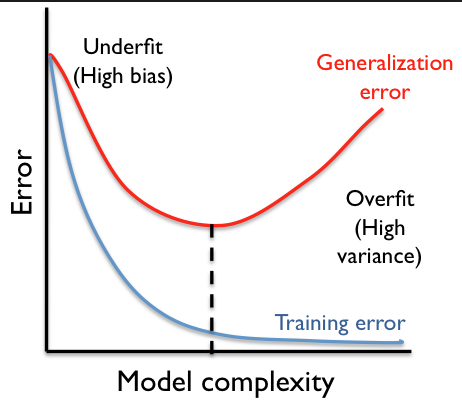
\includegraphics[width=0.5\textwidth]{img/model.png}
\caption{ bias / variance Tradeoff}
\label{fig:bias}
\end{figure}

Some ways of evaluating a model's performance on (some of)  known data are:

\begin{itemize}
\item hold out (just set aside some portion of the data for validation; this is less reliable if the amount of data is small such that the held out portion is very small) 
\item k-fold cross-validation (better than hold out for small datasets) for better visualization  check figure \ref{fig:cross}
\begin{itemize}
\item the training set is divided into k folds
\item iteratively take k$−$1 folds for training and validate on the remaining fold
\item average the results
\item there is also "leave-one-out" cross-validation which is k-fold cross-validation where k=n (n is the number of data points)
\end{itemize}

\begin{figure}[H]
\centering
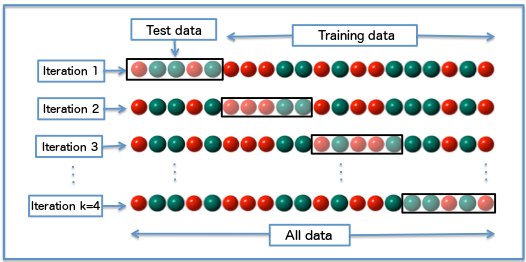
\includegraphics[width=1.0\textwidth]{img/cross.jpg}
\caption{K-cross validation }
\label{fig:cross}
\end{figure}


\item bootstrapping : 
\begin{itemize}
\item new datasets are generated by sampling with replacement (uniformly at random) from the original dataset
\item then train on the bootstrapped dataset and validate on the unselected data
\end{itemize}
\item jackknife resampling : 
essentially to leave-one-out cross-validation, since leave-one-out is basically sampling without replacement
\end{itemize}

\subsection{Evaluating classification models}\label{eva}

here is some important quantities we need to know in order to evaluate a model :
\begin{itemize}
\item Sensitivity: $ \frac{TP}{TP+FN}$ 
\item Specificity: $\frac{TN}{TN+FP}$
\item Positive predictive value:  $\frac{TP}{TP+FP}$ 
\item Negative predictive value: $\frac{TN}{TN+FN}$
\item Accuracy : $\frac{TP+TN}{TP+FP+TN+FN}$
\end{itemize}

\subsubsection{Area under the curve (AUC)}

This method is for binary classification and multilabel classification. In binary classification we may choose some cutoff above which we assign a sample to one class, and below which we assign a sample to the other class.Depending on our cutoff, we will get different results - there is a trade off between the true and false positive rates.\\
we can plot a Receiver Operating Characteristic (ROC) curve, which has for its y-axis \textbf{P(TP)}  and for its x-axis \textbf{P(FP)} . Every point on the curve corresponds to a cutoff value. That is, the ROC curve visualizes a sweep through all the cutoff thresholds so we can see the performance of our classifier across all cutoff thresholds, whereas other metrics (such as the F-score and so on) only tell we the performance for one particular cutoff. By looking at all thresholds at once, we get a more complete and honest picture of how our classifier is performing, in particular, how well it is separating the classes. It is insensitive to the bias of the data's classes - that is, if there are way more or way less of the positive class than there are of the negative class (other metrics may be deceptively favorable or punishing in such unbalanced circumstances).

The area under the curve (AUC) is used to quantify how good the classification algorithm is. In general, an AUC of above 0.8 is considered "good". An AUC of 0.5 (a straight line) is equivalent to random guessing.  


\begin{figure}[H]
\centering
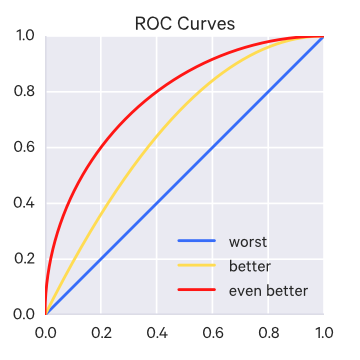
\includegraphics[width=0.5\textwidth]{img/roc.jpg}
\caption{ ROC curves }
\label{fig:bias2}
\end{figure}
So ROC curves (and the associated AUC metric) are very useful for evaluating binary classification.\\Note that ROC curves can be extended to classification of three or more classes by using the one-vs-all approach \\

\textbf{AUC incorporate the explanation below as well :}
AUC is a metric for binary classification and is especially useful when dealing with high-bias data, that is, where one class is much more common than the other. Using accuracy as a metric falls apart in high-bias datasets: for example, say ou have 100 training examples, one of which is is positive, the rest of which are negative. we could develop a model which just labels every thing negative, and it would have 99\% accuracy. So accuracy doesn't really tell  enough here.\\Many binary classifies output some continuous value (0-1), rather than class labels; there is some threshold (usually 0.5) above which one label is assigned, and below which the other label is assigned. Some models may work best with a different threshold. Changing this threshold leads to a trade off between true positives and false positives - for example, decreasing the threshold will yield more true positives, but also more false positives.\\AUC runs over all thresholds and plots the the true vs false positive rates. This curve is called a receiver operating characteristic curve, or ROC curve. A random classifier would give we equal false and true positives, which leads to a AUC of 0.5; the curve in this case would be a straight line. The better the classifier is, the more area under the curve there is (so the AUC approaches 1).

\subsubsection{Confusion Matrices}
This method is suitable for binary or multiclass classification.

For classification, evaluation often comes in the form of a confusion matrix.

The core values are:
\begin{itemize}
\item True positives (TP): samples classified as positive which were labeled positive
\item True negatives (TN): samples classified as negative which were labeled negative
\item False positives (FP): samples classified as positive which were labeled negative
\item False negatives (FN): samples classified as negative which were labeled positive\\

\texttt{A few other metrics are computed from these values }:\\

\item Accuracy: How often is the classifier correct  $\frac{\text{TP} + \text{TN}}{\text{total}}$

\item Misclassification rate (or "error rate"): How often is the classifier wrong $\frac{\text{FP} + \text{FN}}{\text{total}} = 1 $-$ \text{accuracy}$

\item Recall (or "sensitivity" or "true positive rate"): How often are positive-labeled samples predicted as positive $\frac{\text{TP}}{\text{num positive-labeled examples}}$

\item False positive rate: How often are negative-labeled samples predicted as positive  $\frac{\text{FP}}{\text{num negative-labeled examples}}$

\item Specificity (or "true negative rate"): How often are negative-labeled samples predicted as negative  $\frac{\text{TN}}{\text{num negative-labeled examples}}$
\item Precision: How many of the predicted positive samples are correctly predicted   $\frac{\text{TP}}{\text{TP} + \text{FP}}$

\item Prevalence: How many labeled-positive samples are there in the data  $\frac{\text{num positive-labeled examples}}{\text{num examples}}$ \\
Some other values:\\

\item Positive predictive value (PPV): precision but takes prevalence into account. With a perfectly balanced dataset (i.e. equal positive and negative examples, that is prevalence is 0.5), the PPV equals the precision.

\item F-score: The weighted average of recall and precision

\item ohen's Kappa: a measure of how well the classifier performs compared against if it had just guessed randomly, that is a high Kappa score happens when there is a big difference between the accuracy and the null error rate.

\end{itemize}

\subsection{Metric selection}
When it comes to skewed classes (or high bias data), metric selection is more nuanced.

For instance, say we have a dataset where only 0.5\% of the data is in category 1 and the rest is in category 0. we run our model and find that it categorized 99.5\% of the data correctly! But because of the skew in that data, our model could just be: classify each example in category 0, and it would achieve that accuracy.

Note that the convention is to set the rare class to 1 and the other class to 0. That is, we try to predict the rare class.

Instead, we may want to use \textbf{precision/recall} as our evaluation metric.

\begin{figure}[H]
\centering
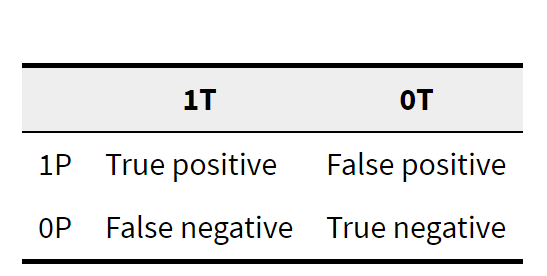
\includegraphics[width=0.6\textwidth]{img/TP.PNG}
\caption{  confusion matrix.}
\label{fig:TP}
\end{figure}

Where 1T/0T indicates the actual class and 1P/0P indicates the predicted class.\\
\textbf{Precision} is the number of true positives over the total number predicted as positive. That is, what fraction of the examples labeled as positive actually are positive  $\frac{\text{true positives}}{\text{true positives} + \text{false positives}}$ .\\
\textbf{Recall} is the number of true positives over the number of actual positives. That is, what fraction of the positive examples in the data were identified  $\frac{\text{true positives}}{\text{true positives} + \text{false negatives}}$
\newline
\newline
\newline
\section{Conclusion:}

in this chapter we have discussed in detail some of the most Popular classification algorithms in machine learning in general and  in Pattern recognition specifically such As SVM , NN and Finally ANN, Next we studied deffirent Methods for selecting $^{[\ref{ms}]}$ a Model Using K cross validation and bootstraping , and their astonishing role in maximization the performance of a classifier . \\
Finally we walked through some of Evaluation metrics that help us evaluate a model such as Sensitivity , Specificity  Positive Predictive value , Negative Predictive value , Accuracy [\ref{eva} ]. \\
\newline
\newline
IN the next chapter we will review some of the most powerful Descriptors for object recognition .





\appendix


\chapter{Microsoft  Kinect Sensor}

\section{Introduction}

Microsoft released the Kinect device in November 2010 as remote controller for the XBOX gaming console \cite{kinect1}. 
It enables the user to command the XBOX through their voice and body gestures and do not require wearing or using additional accessories to track their movements \cite{kinect1}.
 It features an Red-Green-Blue (RGB) video camera, a depth sensor for 3D representation of environment, multi array microphones for voice recognition and Microsoft software that enables human body recognition \cite{kinect1}. \\
The computer vision society realized that Kinect’s depth sensing capabilities can be used beyond gaming purposes and applications in field of robotics, virtual reality and more started to appear \cite{kinect15}. \\
Kinect drivers that were available for Xbox only, now are available for different platforms such as Linux, Windows and Macintosh. 
On top of them Software Development Kits (SDK) are built, thus enabling development of cross-platform applications.

\subsection{Working  Environment  Introduction }
The system of the present thesis consists of three main components:  Hand Detection,  Finger Identification. and Gesture Recognition.  This system is built upon the Candescent  NUI \cite{d} project,  which is freely available online. The Kinect SDK  framework is used to extract  depth data  from the Kinect sensor. From the depth data,  it is easy to distinguish  the user's hands from the background.  When both  hands are present and at some distance apart,  two hand clusters will be found; otherwise, there is only one cluster. 

\subsection{Kinect's Features }

Hardware The Kinect has one RGB camera, one depth sensor that consist of one Infra-Red (IR) projector and one IR camera, an array of four microphones and a motorized tilt for changing the field of view \cite{kinect15}. These components are shown in \ref{fig:cam2}

\begin{figure}[H]
\centering
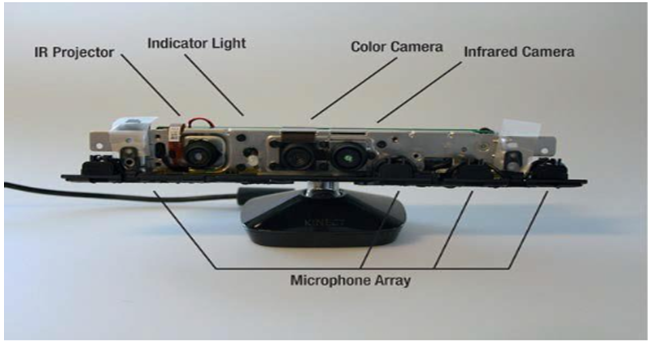
\includegraphics[width=0.53\textwidth]{img/kinectcamera2.png}
\caption{ kinect Hardware }
\label{fig:cam2}
\end{figure}

\textbf{The RGB sensor}  (or video camera) provides 2D view of the scene in three basic colors: Red,Green, and Blue \cite{kinect15} The resolution that can be used is 640x480 pixels or 1280x960 pixels with 32 bits per pixel and the frame rate of 30 frames per second (fps) \cite{kinect15}. \\

\textbf{The depth sensor} \\
– the IR Projector is used to illuminates the scene with structured light while the IR camera observes this illuminated scene and measures the distance of objects from Kinect \cite{kinect15}. As result a depth map is created that gives the distance of objects from the sensor. The depth
map resolution is provided in 320x240 pixels or 640x480 pixels with 16 bits per pixel and an  output frame rate of 30fps \cite{kinect15}. The minimum depth sensor range is from 0.8 meters to a maximum of 4 meters (physical limits). The recommended distance (“Sweet spot” in figure 2.6) is between 1.2m and 3.5m and distances beyond 4m are not recommended since noise get larger \cite{kinect17}. Sun light interferes with infrared light, therefore the depth sensor is not well suited for applications in direct sun light conditions (outdoors)\cite{kinect17} .  

\begin{figure}[H]
\centering
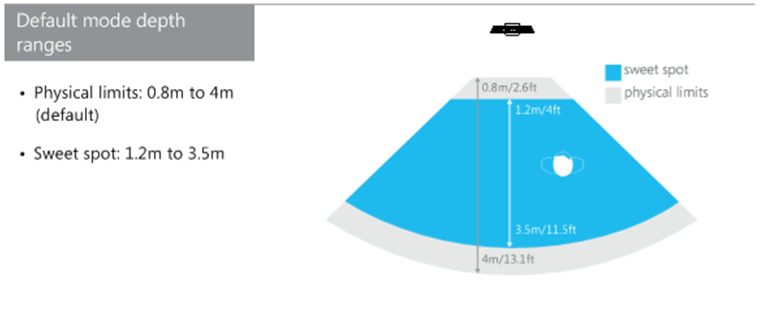
\includegraphics[width=0.8\textwidth]{img/afterworking1.png}
\caption{Kinect depth sensor capabilities}
\label{fig:cam3}
\end{figure}

`\textbf{The motorized tilt}\\
 is used to control the field of view as shown in figure \ref{fig:cam4} and it characteristics are \cite{kinect15} : 
 
\begin{itemize}
\item  Horizontal field of view: 57.5 degree,
\item  Vertical field of view: 43.5 degree,
\item Tilt range: -27 to +27 degree range up and down.

\end{itemize}

\begin{figure}[H]
\centering
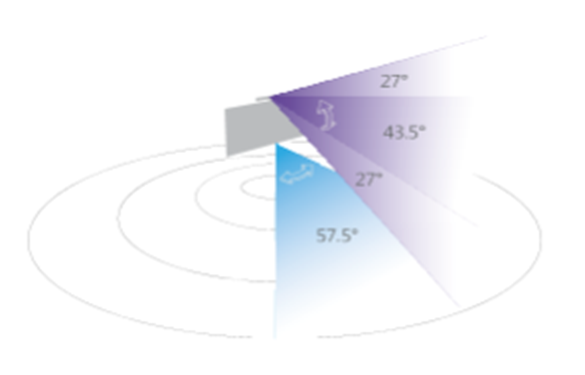
\includegraphics[width=0.6\textwidth]{img/afterworking2.png}
\caption{Kinect depth sensor capabilities}
\label{fig:cam4}
\end{figure}

\textbf{The microphone array} \\
is used for capturing sounds and usually used for speech recognition. It consist of four microphones that enable detection of sound’s source and direction of audio wave \cite{kinect15}. One of them is located at the left of IR projector and the other three microphones are evenly spaced and located at the right of IR camera as shown in \ref{fig:cam5}. The sensor can detect sounds in range of -/+ 50 degree in front of it (\ref{fig:cam5}.a), sound direction in 10 increments  (\ref{fig:cam5}.b) , and offers 20dB (decibel) ambient noise cancellation (\ref{fig:cam5}.c)\cite{kinect17}.

\begin{figure}[H]
\centering
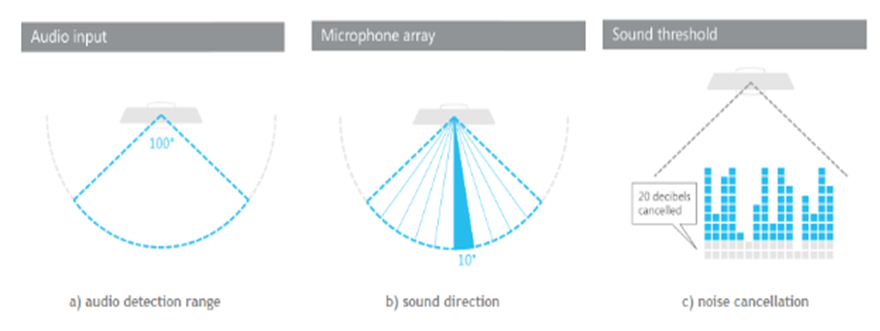
\includegraphics[width=0.8\textwidth]{img/afterworking3.png}
\caption{Kinect sound sensor capabilities a) audio range detection b) sound direction localization c) ambient noise cancellation .
}
\label{fig:cam5}
\end{figure}


\textbf{Skeletal tracking }\\
Skeletal tracking is offered through depth camera. Up to six people can be tracked, while the full skeleton is provided only for two. In full skeleton tracking mode, 20 joints are tracked while in seated mode, half of them (10 joints).The accuracy is larger when the user stands in front of the Kinect, while side standing poses some challenges. Skeletal tracking and two modes are  illustrated in \ref{fig:cam6}.

\begin{figure}[H]
\centering
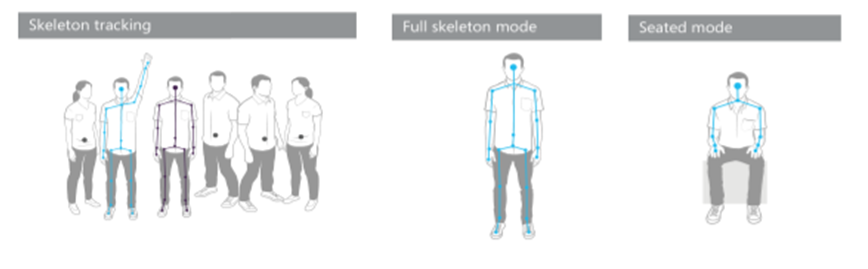
\includegraphics[width=1.0\textwidth]{img/afterworking4.png}
\caption{Skeleton tracking modes through Kinect }
\label{fig:cam6}
\end{figure}

The tracked joint positions are shown in \ref{fig:cam77}
\begin{figure}[H]
\centering
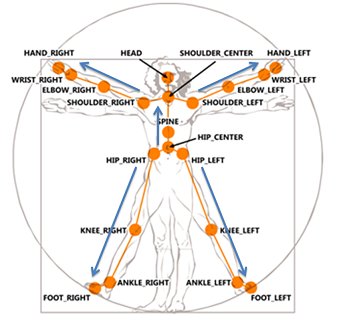
\includegraphics[width=0.4555\textwidth]{img/afterworking5.png}
\caption{Skeleton joint positions offered  through Kinect }
\label{fig:cam77}
\end{figure}

Each skeleton position (body center) and each joint is provided in 3D (x, y, z) coordinates as 
shown in \ref{fig:cam7}. The Kinect is placed at the origin of coordinative system and from Kinect viewpoint: positive Z-axis increases towards the user, positive  Y-axis increases upward and positive  X-axis increases to the left .  

\begin{figure}[H]
\centering
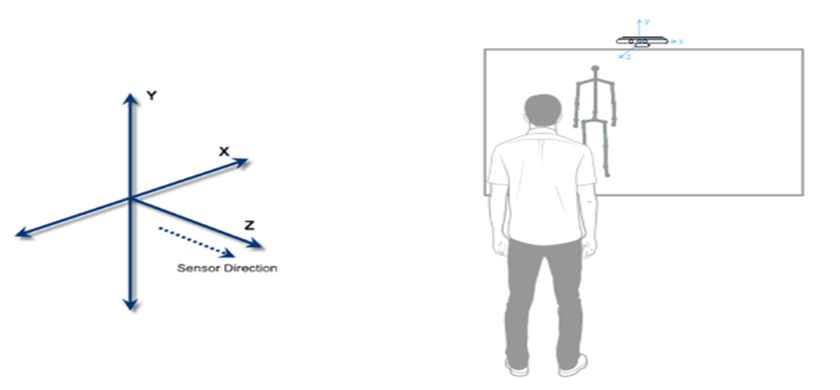
\includegraphics[width=0.7\textwidth]{img/afterworking6.png}
\caption{kinect skeleton coordinate system  }
\label{fig:cam7}
\end{figure}


 
\subsection{linking  kinect SDK with visual studio}

We are using the Kinect SDK version 1.8 and this is how the project is configured. Please note that the developer machine is Windows 7 x86. 
If you are using x64, please change the path accordingly.\\
\textbf{Step 1. } In the Property Manager, right click on the project name and select Add New Project Property\\
Copy C:/Program Files/MicrosoftSDKs/Kinect/v1.0/inc\\
Copy C:/Program Files/MicrosoftSDKs/Kinect/v1.0/lib (you will have both x86 and x64 libraries)\\
\textbf{Step 2}. Configure the project. \\
C/C++ -$>$ General-$>$ add C:/Program Files/Microsoft SDKs/Kinect/v1.8/inc to your Additional Include Directories\\
Linker -$>$ General -$>$ add" C:/Program Files/Microsoft SDKs/Kinect/v1.8/lib/amd64 "  to your Additional Library Directories (if you are configuring for x64, use the amd64 directory)\\
Linker -$>$ Input -$>$ add "Kinect10.lib" to Additional Dependencies\\
\textbf{Step 3}. Compile\\


\chapter{Opencv}

\section{Introduction }
OpenCV (Open Source Computer Vision Library) is released under a BSD license and hence it’s free for both academic and commercial use. It has C++, C, Python and Java interfaces and supports Windows, Linux, Mac OS, iOS and Android. OpenCV was designed for computational efficiency and with a strong focus on real-time applications. Written in optimized C/C++, the library can take advantage of multi-core processing. Enabled with OpenCL, it can take advantage of the hardware acceleration of the underlying heterogeneous compute platform. 
\subsection{Build and install Opencv with Opencv Contrib}

\begin{enumerate}
\item Download CMAKE.
 \url{https://cmake.org/download/}
\item Install Visual studio 2017 Community, with C++ and C support.
\item download Opencv 3.2.0 and opencv\_contrib-3.2.0.
\item launch CMake application and then specify the source and build directory as shown in figure below. The red box must be filled with the directory path of OpenCV source, and the green box must be filled with the directory path of designated build folder.

\begin{figure}[H]
\centering
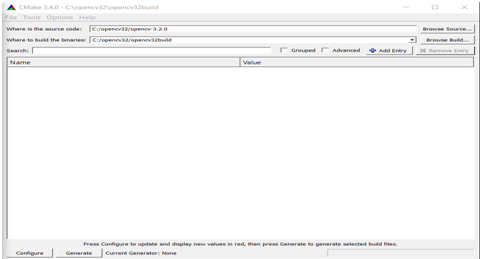
\includegraphics[width=0.9\textwidth]{img/working1.png}
\caption{ setting Cmake right directories }
\label{fig:working1}
\end{figure}

\item we can hit several times  configure. Until we have some list of possible settings like on image below. Use different settings and configuration options. choose  solution we want. FFMPEG, OPENCL support and \textbf{generate OPENCV.SLN file inside  opencv3.0 build folder.} 

\begin{figure}[H]
\centering
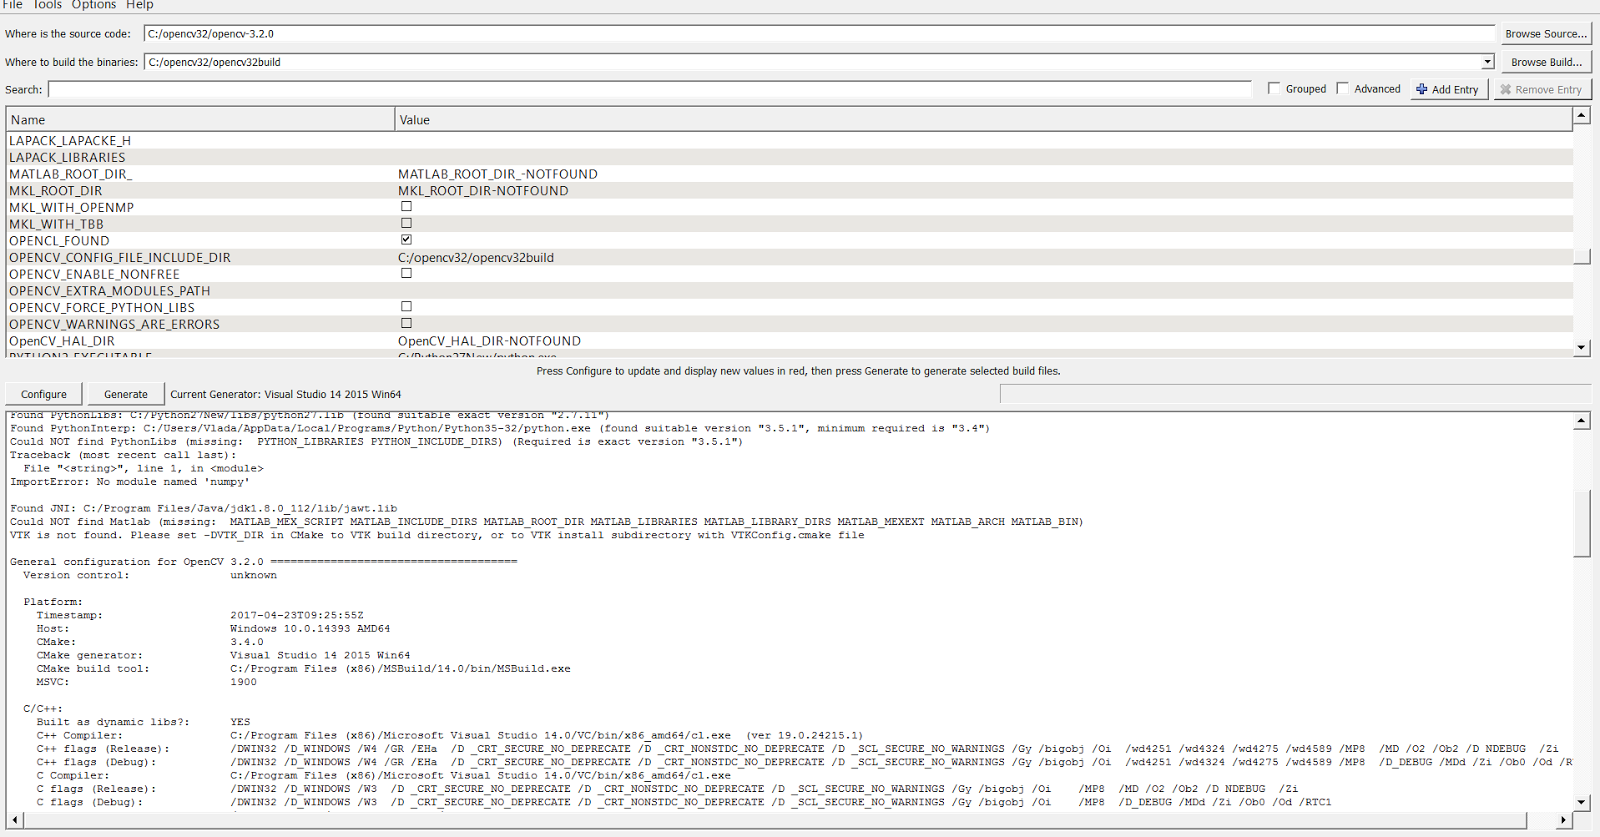
\includegraphics[width=0.9\textwidth]{img/working2.png}
\caption{ result after building }
\label{fig:working2}
\end{figure}

\item FIRST just select DEBUG, x64 version like on picture, click right mouse on Entire solution and hit BUILD the  solution should look like on the next figure . 
\begin{figure}[H]
\centering
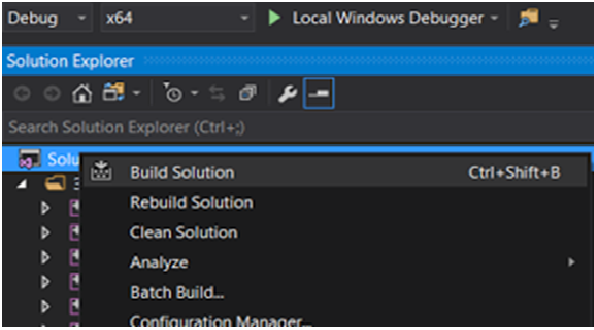
\includegraphics[width=0.6\textwidth]{img/working3.png}
\caption{ building solution}
\label{fig:working3}
\end{figure}

\item 	Second you need to switch from DEBUG to RELEASE and build the solution again. \textbf{This build} also Cmake target install, (you can see this under install) where  your installation is located. \\
Your installation location usually is under opencv32build/install .


\end{enumerate}

\newpage

\subsection{linking Visual studio with opencv :}

\begin{enumerate}
\item OpenCV visual studio and create a console application 
\item in configuration Properties -$> C/C++ $-$>$ Additional Include Directories , then add OpenCV's Includes folders :
 \begin{itemize}
     \item C:/opencv/build/include
     \item C:/opencv/build/include/opencv
     \item C:/opencv/build/include/opencv2
   \end{itemize}
\item in configuration Properties -$>Linker$-$>$Additional Library Directories -$> $ add folder lib of OpenCV :\\
     C:/opencv/build/x64/vc14/lib 
\item in configuration Properties$->$ Linker$->$Additional Dependence$->$ add folder lib of OpenCV .
 \begin{itemize}
     \item opencv\_world320d.lib
     \item opencv\_features2d320d.lib
     \item opencv\_xfeatures2d320d.lib
   \end{itemize}

\end{enumerate}





%%%%%%%%%%%%%%%%%%%%%%%%%%%%%%%%%%%%%%%%%%%%%%%%%%%%%%%%%%%%%%%%%%%%%%%%%%%%%%%%%%%%%%%%%%%%%%%%%%%%%%%%%
\medskip



\begin{thebibliography}{80}

\bibitem{0}
 Antonis  A Argyros  and  Manolis I A Lourakis.   Binocular  hand  tracking  and reconstruction  based on 2d shape matching. CPR, pages 207- 210, 2006.
\bibitem{1}
 P.  Buehler,  M. Everingham,  D. P. Huttenlocher,  and A. Zisserman.  Long term arm and hand  tracking  for continuous sign language TV broadcasts.   In British Machine  Vision Conference, 2008.
\bibitem{2}   The  Duy Bui and Long Thang Nguyen. Recognizing postures in vietnamese sign language with MEMS accelerometers.  Iece Sensors Journal, 7(5):707712, 2007.
\bibitem{3}
  Helen Cooper and Richard Bowden. Large lexicon detection  of sign language.  In

ICCV,  Workshop Human  Comp. Inter, 2007.

\bibitem{4}
   P Dreuw,  T Deselaers, D Ryba.ch, D Keysers,  and H Ney. Tracking using dynamic programming  for appearance-based  sign language recognition.  7th Internotional Conference on Automatic  Face and Gesture Recognition FGR06, 62(1):293-298,
2006.

\bibitem{5}
   Philippe Dreuw, Jens Forster, and Hermann Ney.  Tracking benchmark databases for video-based sign language recognition.  In ECCV  International  Workshop on Sign Gesture and Activity  SCA  Crete Greece September 2010, 2010.
\bibitem{6}
  Philippe  Dreuw,   Carol  Neidle,   Vassilis Athitsos,    Stan  Sclaroff, and  Hermann Ney. Benchmark databases  for video-based automatic  sign language recognition. Pattern  Recognition, pages 6--6, 2008.
\bibitem{7}
  R L Graham.   An efficient algorithm  for determining  the convex hull of a finite planar  set.  Information  Processing Letters, 1(4):132--133, 1972. 
\bibitem{700}
  Y  Han.    A  low-cost  visual   motion   data   glove  as  an  input   device  to  interpret human   hand  gestures.   Ieee Trans Consum Electron, 56(2):501-509, 2010.
\bibitem{8}
  Guan-Feng He, Sun-Kyung Kang, Won-Chang Song, and Sung-Tae Jung.  Real- time gesture recognition using 3D depth  camera.  In Software Engineering and Service Science  (ICSESS),  2011 IEEE  2nd International  Conference on, pages
187 -190, 2011.

\bibitem{9}
  Jos L. Hernndez-rebollar,  Robert V. Lindeman, and Nicholas Kyriakopoulos. A multi-class pattern  recognition system for practical finger spelling translation.  In In Proceedings of the 4th IEEE  International  Conference on Multimodal Inter- faces, pages 185-190, 2002.
\bibitem{10}
  Holger Kenn,  Friedrich Van Megen, and  Robert  Sugar.  A glove-based gesture interface  for wearable  computing  applications.    Applied  Wearable Computing
(IFAWC),  2007 4th International  Forum on, pages 1  --10,   2007.
'                   '

\bibitem{11}
  Ji-Hwan Kim, Nguyen Due Thang, and Tae-Seong Kim. 3-D hand motion tracking and gesture recognition using a data  glove. In Itulustrial Electronics, 2009. ISIE  2009. IEEE  International  Symposium  on, pages 1013 -1018, 2009.
\bibitem{12}
 H Nanda and K Fujimura.  Visual tracking using depth  data.   2004 Conference on Computer  Vision and Pattern  Recognition Workshop, OO(C):37-37, 2004.
\bibitem{13}
   Eng-Jon Ong and Richard Bowden. A boosted classifier tree for hand shape de- tection.   In Proceedings of the Sixth IEEE international conference on Automatic face  and gesture recognition, FGR'  04, pages 889-894, Washington,  DC, USA,
2004. IEEE Computer  Society.

\bibitem{14}
  OpenNI organization.  OpenNI User Guide, 2010. Last viewed 19-01-2011 11:32. 
\bibitem{140}
 Jagdish   L Raheja,   Ankit  Chaudhary,    and  Kunal   Singal.   Tracking   of fingertips and  centers   of palm  using  KINECT.     2011 Third International  Conference on Computational Intelligence Modelling Simulation, pages  248--252, 2011.
\bibitem{15}
 T Starner,   J  Weaver,  and  A Pentland.    Real-time   american   sign language   recog- nition   using  desk  and  wearable   computer   based  video.   IEEE  Transactions on Pattern  Analysis  and Machine Intelligence, 20(12):1371-1375,    1998.
\bibitem{16}
 Stefan   Stegrnueller.     Hand   and  finger  tracking   with   Kinect   depth   data,   2011.

\url{http://candescentnui.codeplex.com}.

\bibitem{17}
 K N Tarchanidis   and  J  N Lygouras.   Data  glove with  a force sensor,  2003.

\bibitem{18}
   M. Van den  Bergh  and  L. Van Cool.  Combining   RGB  and  ToF  cameras  for real- time  3D hand  gesture  interaction.    In Applications of Computer Vision (WACV),
2011 IEEE  Workshop on, pages  66 -72,  2011.

\bibitem{19}
 Cheoljong   Yang,  Yujeong  Jang,   Jounghoon   Beh,  David  Han,  and  Hanseok  Ko. Gesture   recognition   using  depth-based    hand   tracking   for  contactless   controller application.    In  Consumer Electronics (ICCE), 2012 IEEE International  Confer- ence on, pages  297 -298,  2012

\bibitem{20}D. S. Zhang and G. J. Lu. A Comparative Study on Shape Retrieval
Using Fourier Descriptors with Different Shape Signatures. In Proc. Int.
Conference on Multimedia and Distance Education. Fargo, ND, USA,
pp.1-9, June 2001. 
\bibitem{21}
Kai Guo; Ishwar, P.; Konrad, J., "Action Recognition in Video by Covariance
Matching of Silhouette Tunnels," Computer Graphics and Image Processing
(SIBGRAPI), 2009 XXII Brazilian Symposium on , vol., no., pp.299,306, 11-15 Oct.
2009 

\bibitem{AA}Leutenegger, Stefan, Margarita Chli, and Roland Y. Siegwart. “BRISK: Binary Robust
Invariant Scalable Keypoints.” International Conference on Computer Vision, 2011.

\bibitem{b} K. Ha, Y. Abe, Z. Chen, W. Hu, B. Amos, P. Pillai, and M. Satya- narayanan, “Adaptive vm handoff across cloudlets,” Technical Report CMU-CS-15-113, CMU School of Computer Science, Tech. Rep., 2015.

\bibitem{c} S. K. Bose, S. Brock, R. Skeoch, and S. Rao, “Cloudspider: Combining replication with scheduling for optimizing live migration of virtual machines across wide area networks,” in Cluster, Cloud and Grid Computing (CCGrid), 2011 11th

\bibitem{AAA}  Gleason, Josh, BRISK (Presentation by Josh Gleason) at International Conference on
Computer Vision, 2011.

\bibitem{d}  Ms. Lopa J. Vora “International Journal of Modern Trends in Engineering and Research (IJMTER)“ evol Volume 02, Issue 10, [October – 2015] ISSN (Online):2349–9745 ; ISSN (Print):2393-8161

\bibitem{MM} Tuytelaars, T., Mikolajczyk, K.: Local invariant feature detectors: a survey. Found. Trends
Comput. Graph. Vis. 3(3), 177–280 (2007)

\bibitem{j}  Ito, Minami, Hiroshi Tamura, Ichiro Fujita, and Keiji
Tanaka, “Size and position invariance of neuronal responses
in monkey inferotemporal cortex,”
Journal of Neurophysiol-
ogy, 73, 1 (1995), pp. 218–226.


\bibitem{f} Crowley, James L., and Alice C. Parker, “A representation
for shape based on peaks and ridges in the difference of lowpass
transform,”
IEEE Trans. on Pattern Analysis and Ma-
chine Intelligence,
6, 2 (1984), pp. 156–170.

\bibitem{e}Lindeberg, Tony, “Detecting salient blob-like image structures and their scales with a scale-space primal sketch:
a method for focus-of-attention,”
International Journal of
Computer Vision,
11, 3 (1993), pp. 283–318.



\bibitem{h} Oliva, A., Torralba, A.: Modeling the shape of the scene: a holistic representation of the spatial
envelope. Int. J. Comput. Vis. 42(3), 145–175 (2001)
\bibitem{i} Bianco, S., Mazzini, D., Pau, D., Schettini, R.: Local detectors and compact descriptors for
visual search: a quantitative comparison. Digital Signal Process. 44, 1–13 (2015)
\bibitem{k} Jégou, H., Perronnin, F., Douze, M., Sánchez, J., Pérez, P., Schmid, C.: Aggregating local
descriptors into a compact codes. IEEE Trans. Pattern Anal. Mach. Intell. 34(9), 1704–1716
(2012)
\bibitem{kinect}
Microsoft, “Kinect for Windows Sensor Components and Specifications.” [Online]. Available: \url{http://msdn.microsoft.com/en-us/library/jj131033.aspx}Accessed: 06-Dec-2013 ]

\bibitem{kinect1}
 Microsoft, “Kinect Fact Sheet,” 2010. [Online]. Available: \url{www.microsoft.com/enus/news/presskits/xbox/docs/kinectfs.docx}.
\bibitem{kinect15}
M. Andersen, T. Jensen, and P. Lisouski, “Kinect depth sensor evaluation for computer
vision applications,” 2012.
\bibitem{kinect17}
Microsoft, “Kinect for Windows - Human Interface Guidelines.” [Online]. Available:
\url{http://msdn.microsoft.com/en-us/library/jj663791.aspx}.
\bibitem{kinect18}
J. Webb and J. Ashley, Beginning Kinect Programming with the Microsoft Kinect SDK.
Apress, 2012
\bibitem{kinect20}
Microsoft, “Coordinate Space.” [Online]. Available: \url{http://msdn.microsoft.com/enus/library/hh973078.aspx#Depth\_Ranges}.
[Accessed: 06-Dec-2013].

\bibitem{clif}
C. Chan, S. S. Mirfakhrae, “ Hand Gesture Recognition using
Kinect”, Bchelor Thesis, Boston University Department of
Electrical and Computer Engineering ,Boston, Dec 13, 2013.
\bibitem{kmeans}
J. B. MacQueen (1967): "Some Methods for classification and Analysis of Multivariate Observations, Proceedings of 5-th Berkeley Symposium on Mathematical Statistics and Probability", Berkeley, University of California Press, 1:281-297
\bibitem{Arthur} 
Arthur, D.; Vassilvitskii, S. (2007). "k-means++: the advantages of careful seeding" (PDF). Proceedings of the eighteenth annual ACM-SIAM symposium on Discrete algorithms. Society for Industrial and Applied Mathematics Philadelphia, PA, USA. pp. 1027–1035.

\bibitem{svm}
Hill, T.,  Lewicki, P. (2006). Statistics Methods and applications : a comprehensive reference for science, industry, and data mining. Tulsa, Okla: StatSoft.


\end{thebibliography}



\end{document}
